% ============================================================
%  Relatório Técnico — Inspeção Visual Automática de Frutas
%  Visão Computacional — Junho 2026
% ============================================================
\documentclass[12pt,a4paper]{article}
\usepackage[utf8]{inputenc}
\usepackage[T1]{fontenc}
\usepackage[brazil]{babel}
\usepackage{graphicx}
\usepackage{booktabs}
\usepackage{float}
\usepackage{hyperref}
\usepackage{geometry}
\usepackage{amsmath}
\usepackage{caption}
\usepackage{subcaption}
\usepackage{xcolor}
\usepackage{array}
\usepackage{multirow}

\geometry{margin=2.5cm}
\setlength{\parskip}{0.25em}
\setlength{\parindent}{0pt}

\hypersetup{
    colorlinks=true,
    linkcolor=blue!60!black,
    urlcolor=blue!60!black,
}

% ============================================================
\begin{document}

% ── CAPA ─────────────────────────────────────────────────────
\begin{titlepage}
    \centering
    \vspace*{2cm}

    {\LARGE\bfseries Sistema de Inspeção Visual Automática de Frutas\par}
    \vspace{0.4cm}
    {\large Relatório Técnico\,|\,Visão Computacional\par}

    \vspace{1.8cm}
    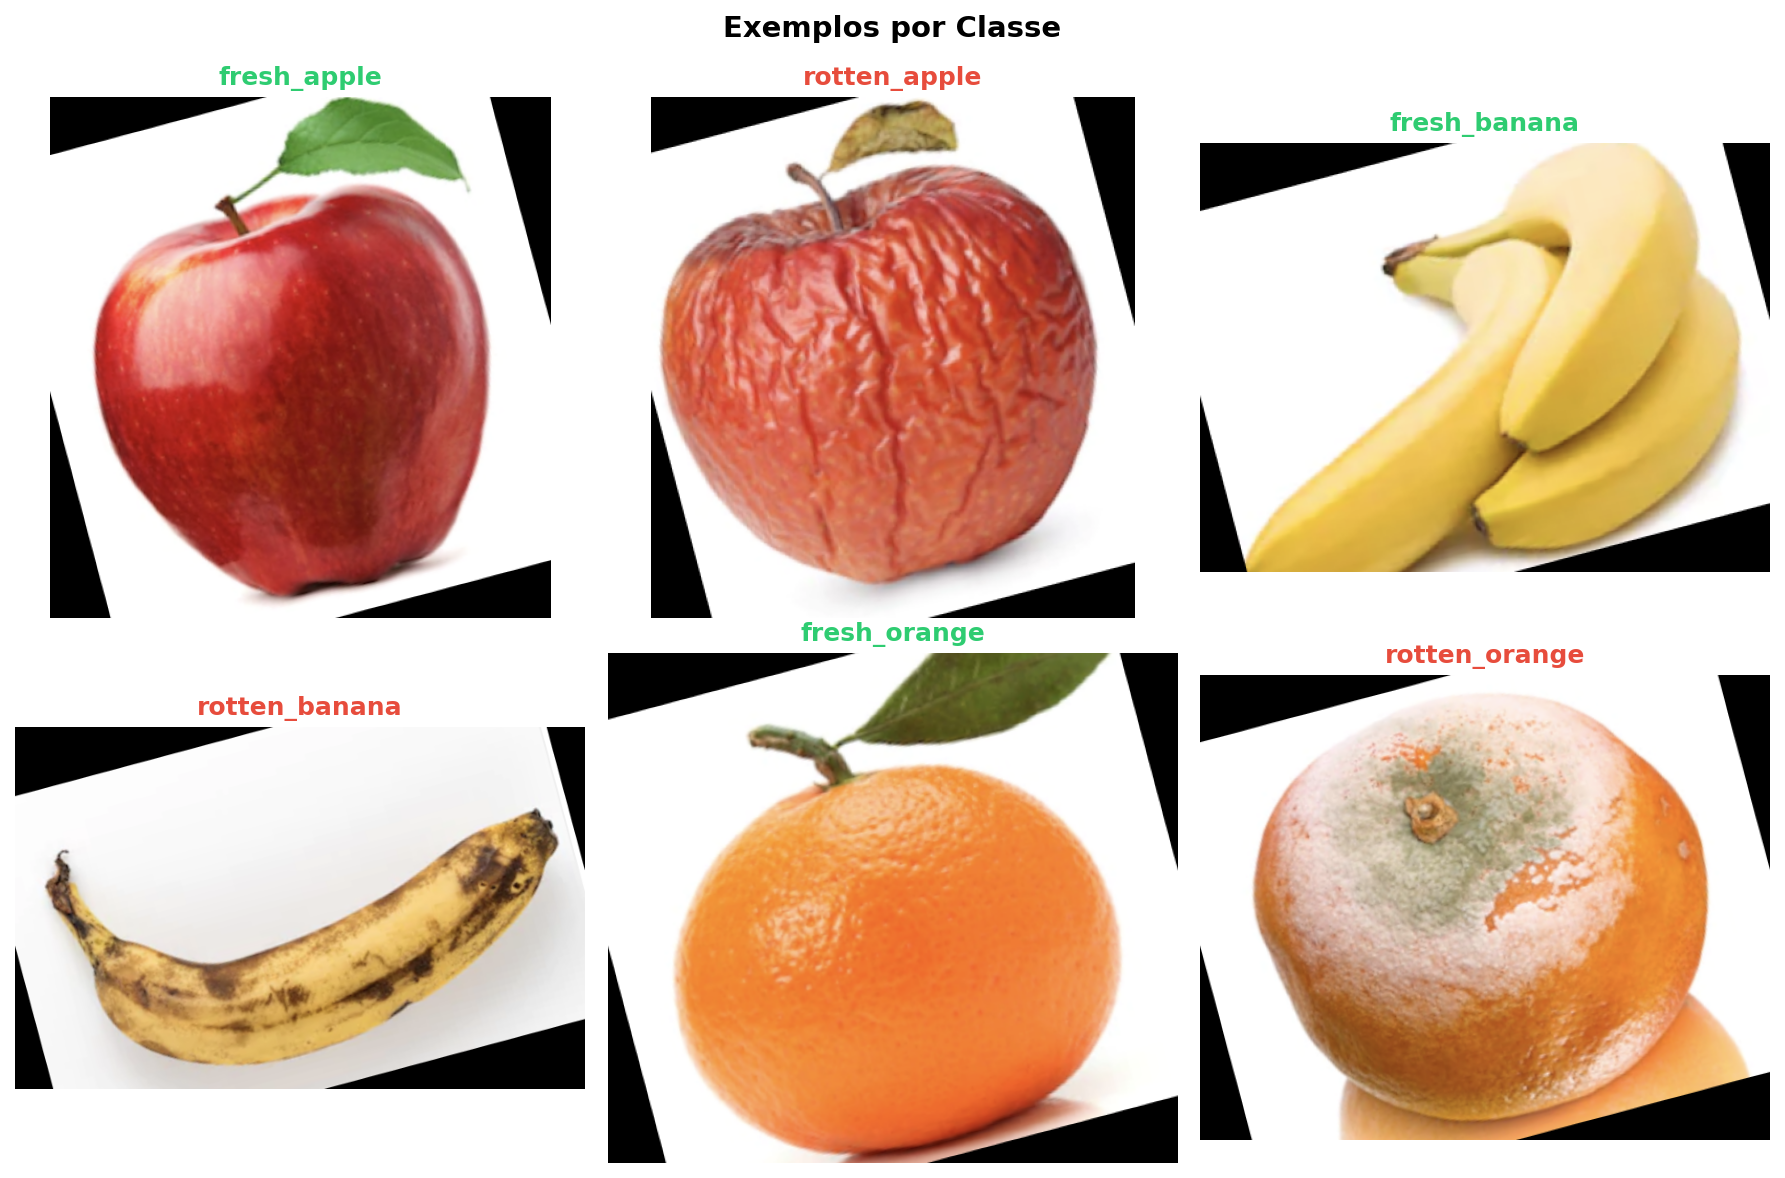
\includegraphics[width=0.52\textwidth]{../outputs/figures/eda_exemplos_por_classe.png}

    \vspace{1.8cm}
    {\large
        Felipe de Mello Vieira\\[0.25em]
        Felipe Yukiya Soares Uemura\\[0.25em]
        Gabriel Sampaio Giacomoni\\[0.25em]
        Leonardo Gabriel Herédia
    \par}

    \vfill
    {\large Junho de 2026\par}
\end{titlepage}

% ── SUMÁRIO ──────────────────────────────────────────────────
\tableofcontents
\bigskip

% ============================================================
\section{Introdução e Dataset}
% ============================================================

A inspeção de qualidade de frutas em centrais de distribuição é realizada manualmente,
processo lento e sujeito a inconsistências. Visão computacional permite automatizar
essa tarefa: a partir de uma imagem RGB, classificar cada fruta como \textit{fresca}
ou \textit{podre} em tempo real.

\textbf{Dataset:} utilizamos o \textit{Fruit Quality Detection}
\href{https://www.kaggle.com/datasets/sriramr/fruits-fresh-and-rotten-for-classification}{(Kaggle)},
com imagens sobre fundo branco controlado. Aplicamos \textit{undersampling} com
$\mathrm{random\_state}{=}42$, obtendo \textbf{1.200 imagens}, \textbf{200 por classe},
em 6 classes: \texttt{fresh\_apple}, \texttt{rotten\_apple}, \texttt{fresh\_banana},
\texttt{rotten\_banana}, \texttt{fresh\_orange}, \texttt{rotten\_orange}.

\textbf{Eliminação de data leakage:} o dataset original continha variantes augmentadas
(\textit{rotated\_by\_15}, \textit{rotated\_by\_30}, \textit{salt\_and\_pepper}).
Um split aleatório colocava variantes da mesma fruta em treino e teste, vazando
${\approx}62\%$ das amostras. Removemos as variantes e revalidamos via \textit{perceptual
hash}: restaram apenas 6 pares próximos em 1.200 imagens (${\approx}0{,}5\%$, desprezível).
As métricas reportadas refletem essa configuração limpa.

\begin{figure}[!htbp]
    \centering
    \begin{subfigure}[b]{0.49\textwidth}
        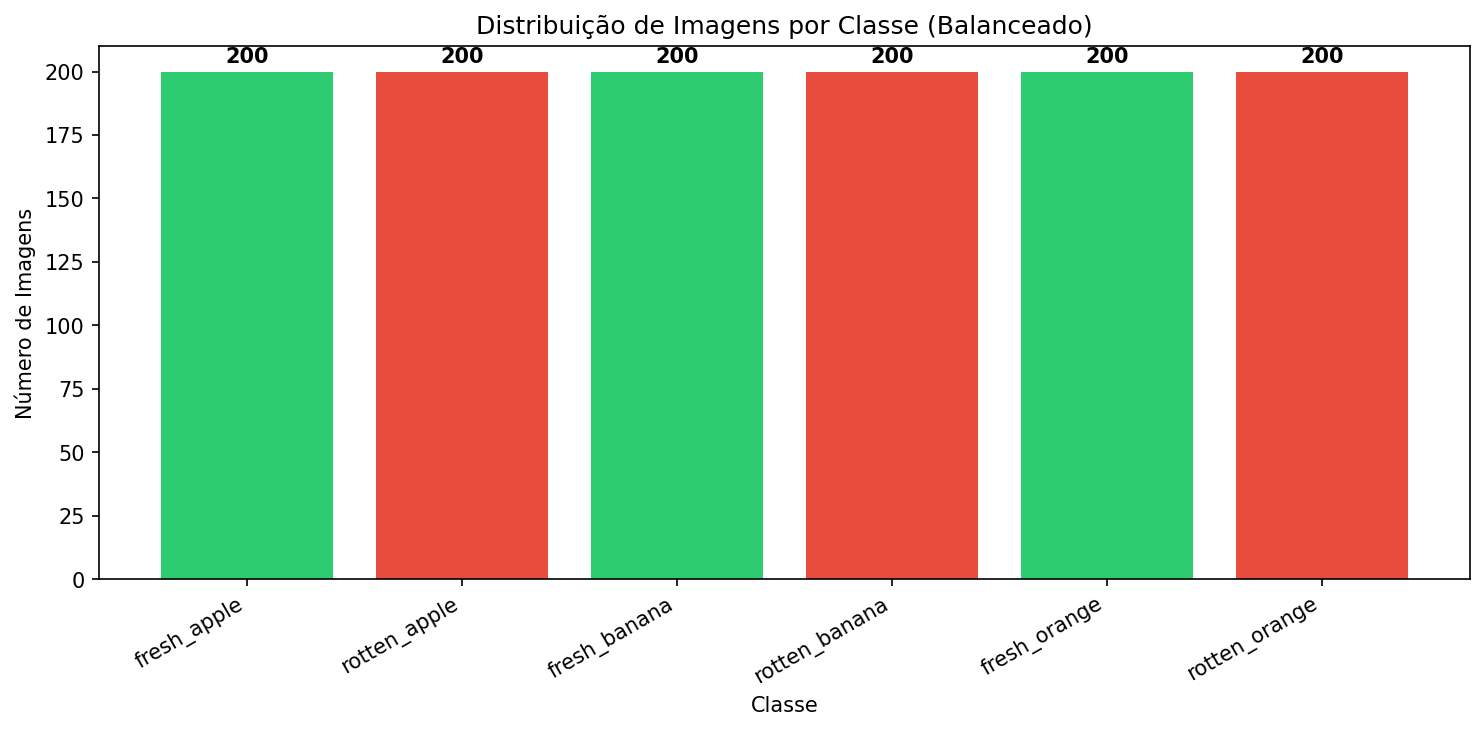
\includegraphics[width=\textwidth]{../outputs/figures/eda_class_distribution.png}
        \caption{Distribuição por classe (balanceada).}
    \end{subfigure}
    \hfill
    \begin{subfigure}[b]{0.46\textwidth}
        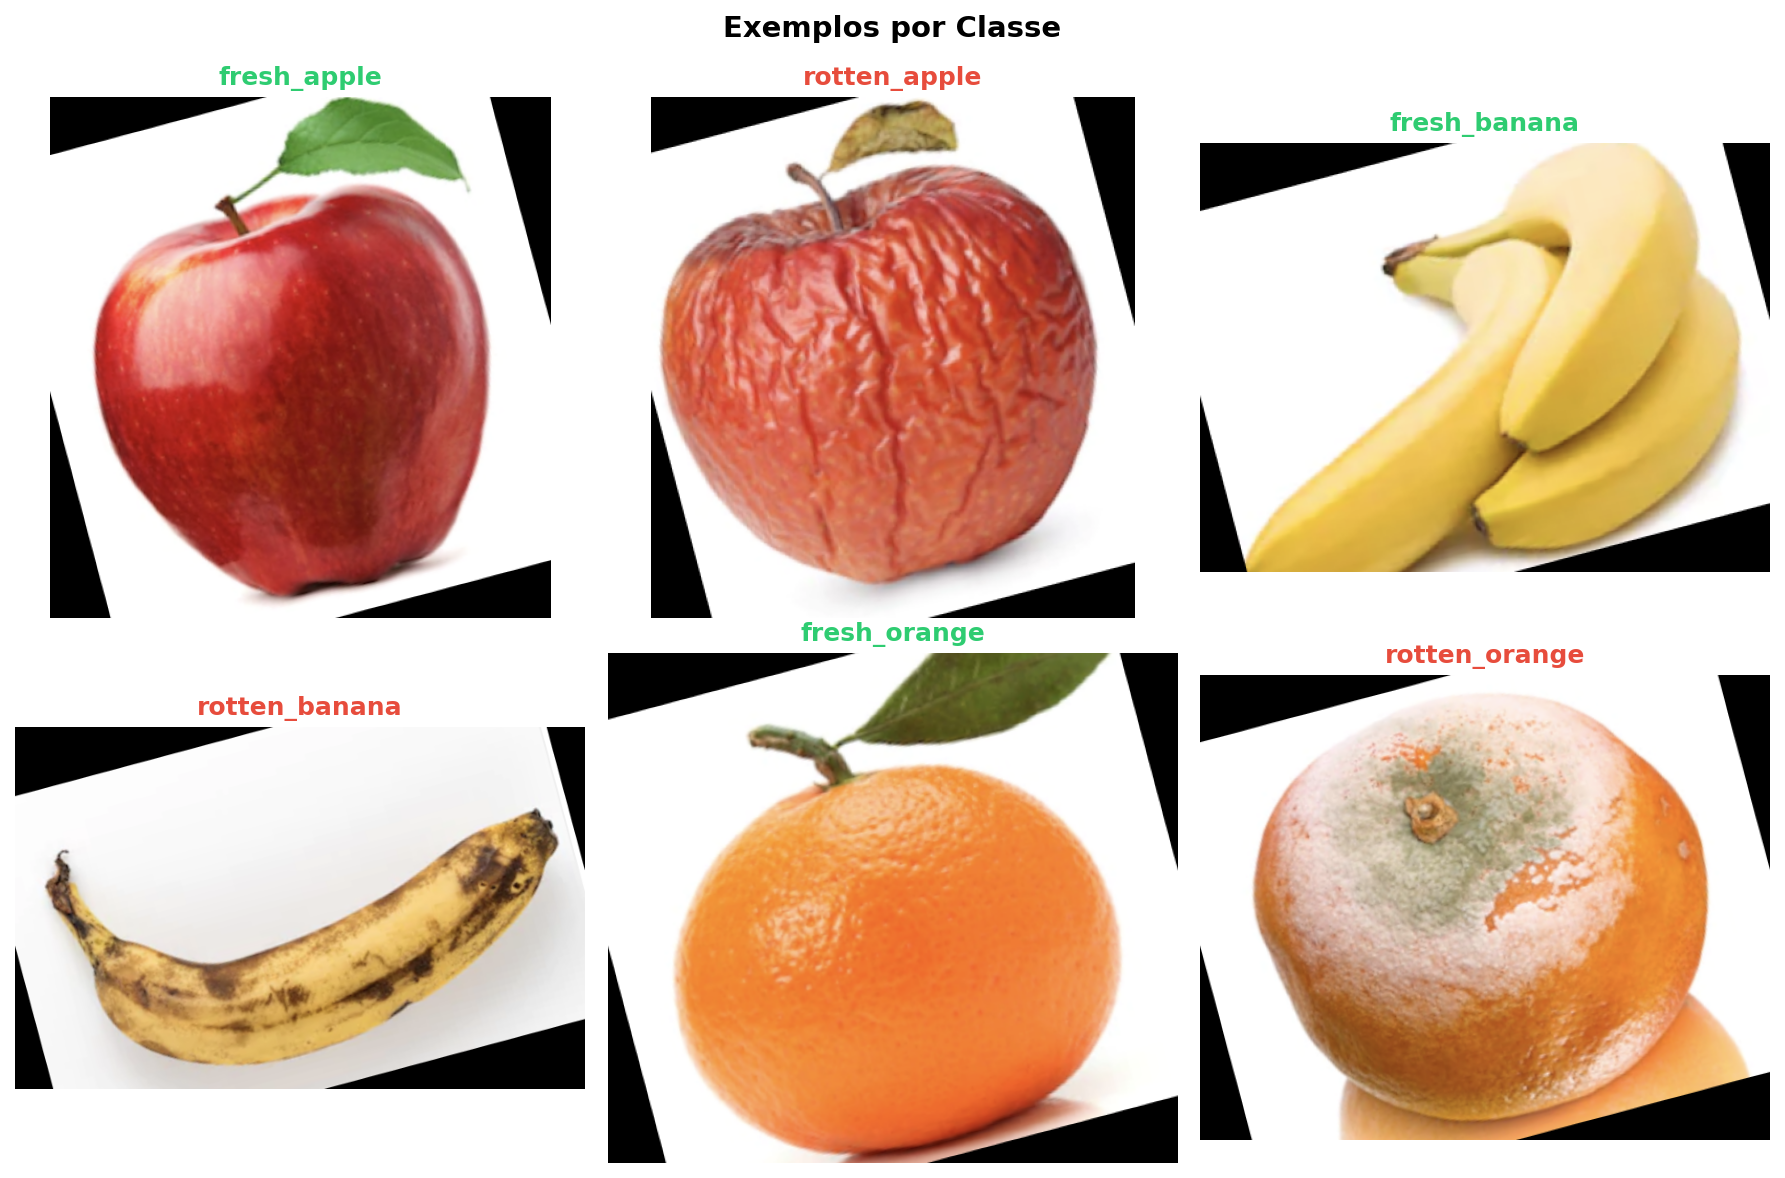
\includegraphics[width=\textwidth]{../outputs/figures/eda_exemplos_por_classe.png}
        \caption{Exemplos de imagens por classe.}
    \end{subfigure}
    \caption{Análise exploratória do dataset (200 imagens/classe, 6 classes).}
    \label{fig:eda}
\end{figure}

% ============================================================
\section{Pipeline Proposto}
% ============================================================

O sistema possui cinco etapas sequenciais. A divisão dos dados segue
\textbf{70\% treino / 15\% validação / 15\% teste}, estratificado por classe.
O \texttt{StandardScaler} é ajustado exclusivamente em $X_{\mathrm{train}}$.

\begin{samepage}
{\small
\begin{verbatim}
  Imagem RGB (fundo controlado)
          |
          v
  [1] Segmentacao Otsu V2 (HSV-S + fallback)  -->  mascara binaria
          |
          v
  [2] Extracao de features:
      Shape(6) + Hu(7) + Cor HSV(22) + GLCM(4) + LBP(26) = 65 features
          |
          v
  [3] Classificador  (RF / SVM / LR  +  GridSearchCV, k=5)
          |
          v
  Predicao: fresh_apple | rotten_apple | fresh_banana | ...
\end{verbatim}
}
\end{samepage}

% ============================================================
\section{Segmentação}
% ============================================================

\textbf{Otsu V2 (escolhido):} aplicamos Otsu no canal de \emph{saturação} (S) do espaço
HSV, explorando o contraste entre fundo branco (saturação baixa) e fruta colorida
(saturação alta). Quando a saturação não discrimina bem (máscara $< 5\%$ ou $> 70\%$),
um fallback aplica Otsu no canal de cinza com detecção automática de inversão
(compara intensidade de borda vs.\ centro). Morfologia com kernel elíptico $5{\times}5$
(erosão + dilatação, 2 iterações) remove ruído; o maior contorno é retido.
\textbf{Zero erros em 1.200 imagens.}

\textbf{Watershed:} usa o canal S como mapa de distância, picos locais como marcadores
e inundação sobre o negativo do mapa. Mais adequado para cenas não controladas com
objetos sobrepostos, mas exige maior parametrização e é sensível a sombras.

\begin{table}[!htbp]
\centering
\caption{Comparação entre Otsu V2 e Watershed.}
\label{tab:seg}
\small
\begin{tabular}{lll}
\toprule
\textbf{Critério} & \textbf{Otsu V2} & \textbf{Watershed} \\
\midrule
Robustez ao fundo controlado & Alta & Média \\
Limpeza da máscara           & Alta & Média (falsos positivos) \\
Parametrização               & Baixa (automática) & Alta \\
Erros em 1.200 imagens       & \textbf{0} & Ocasionais \\
\bottomrule
\end{tabular}
\end{table}

\begin{figure}[!htbp]
    \centering
    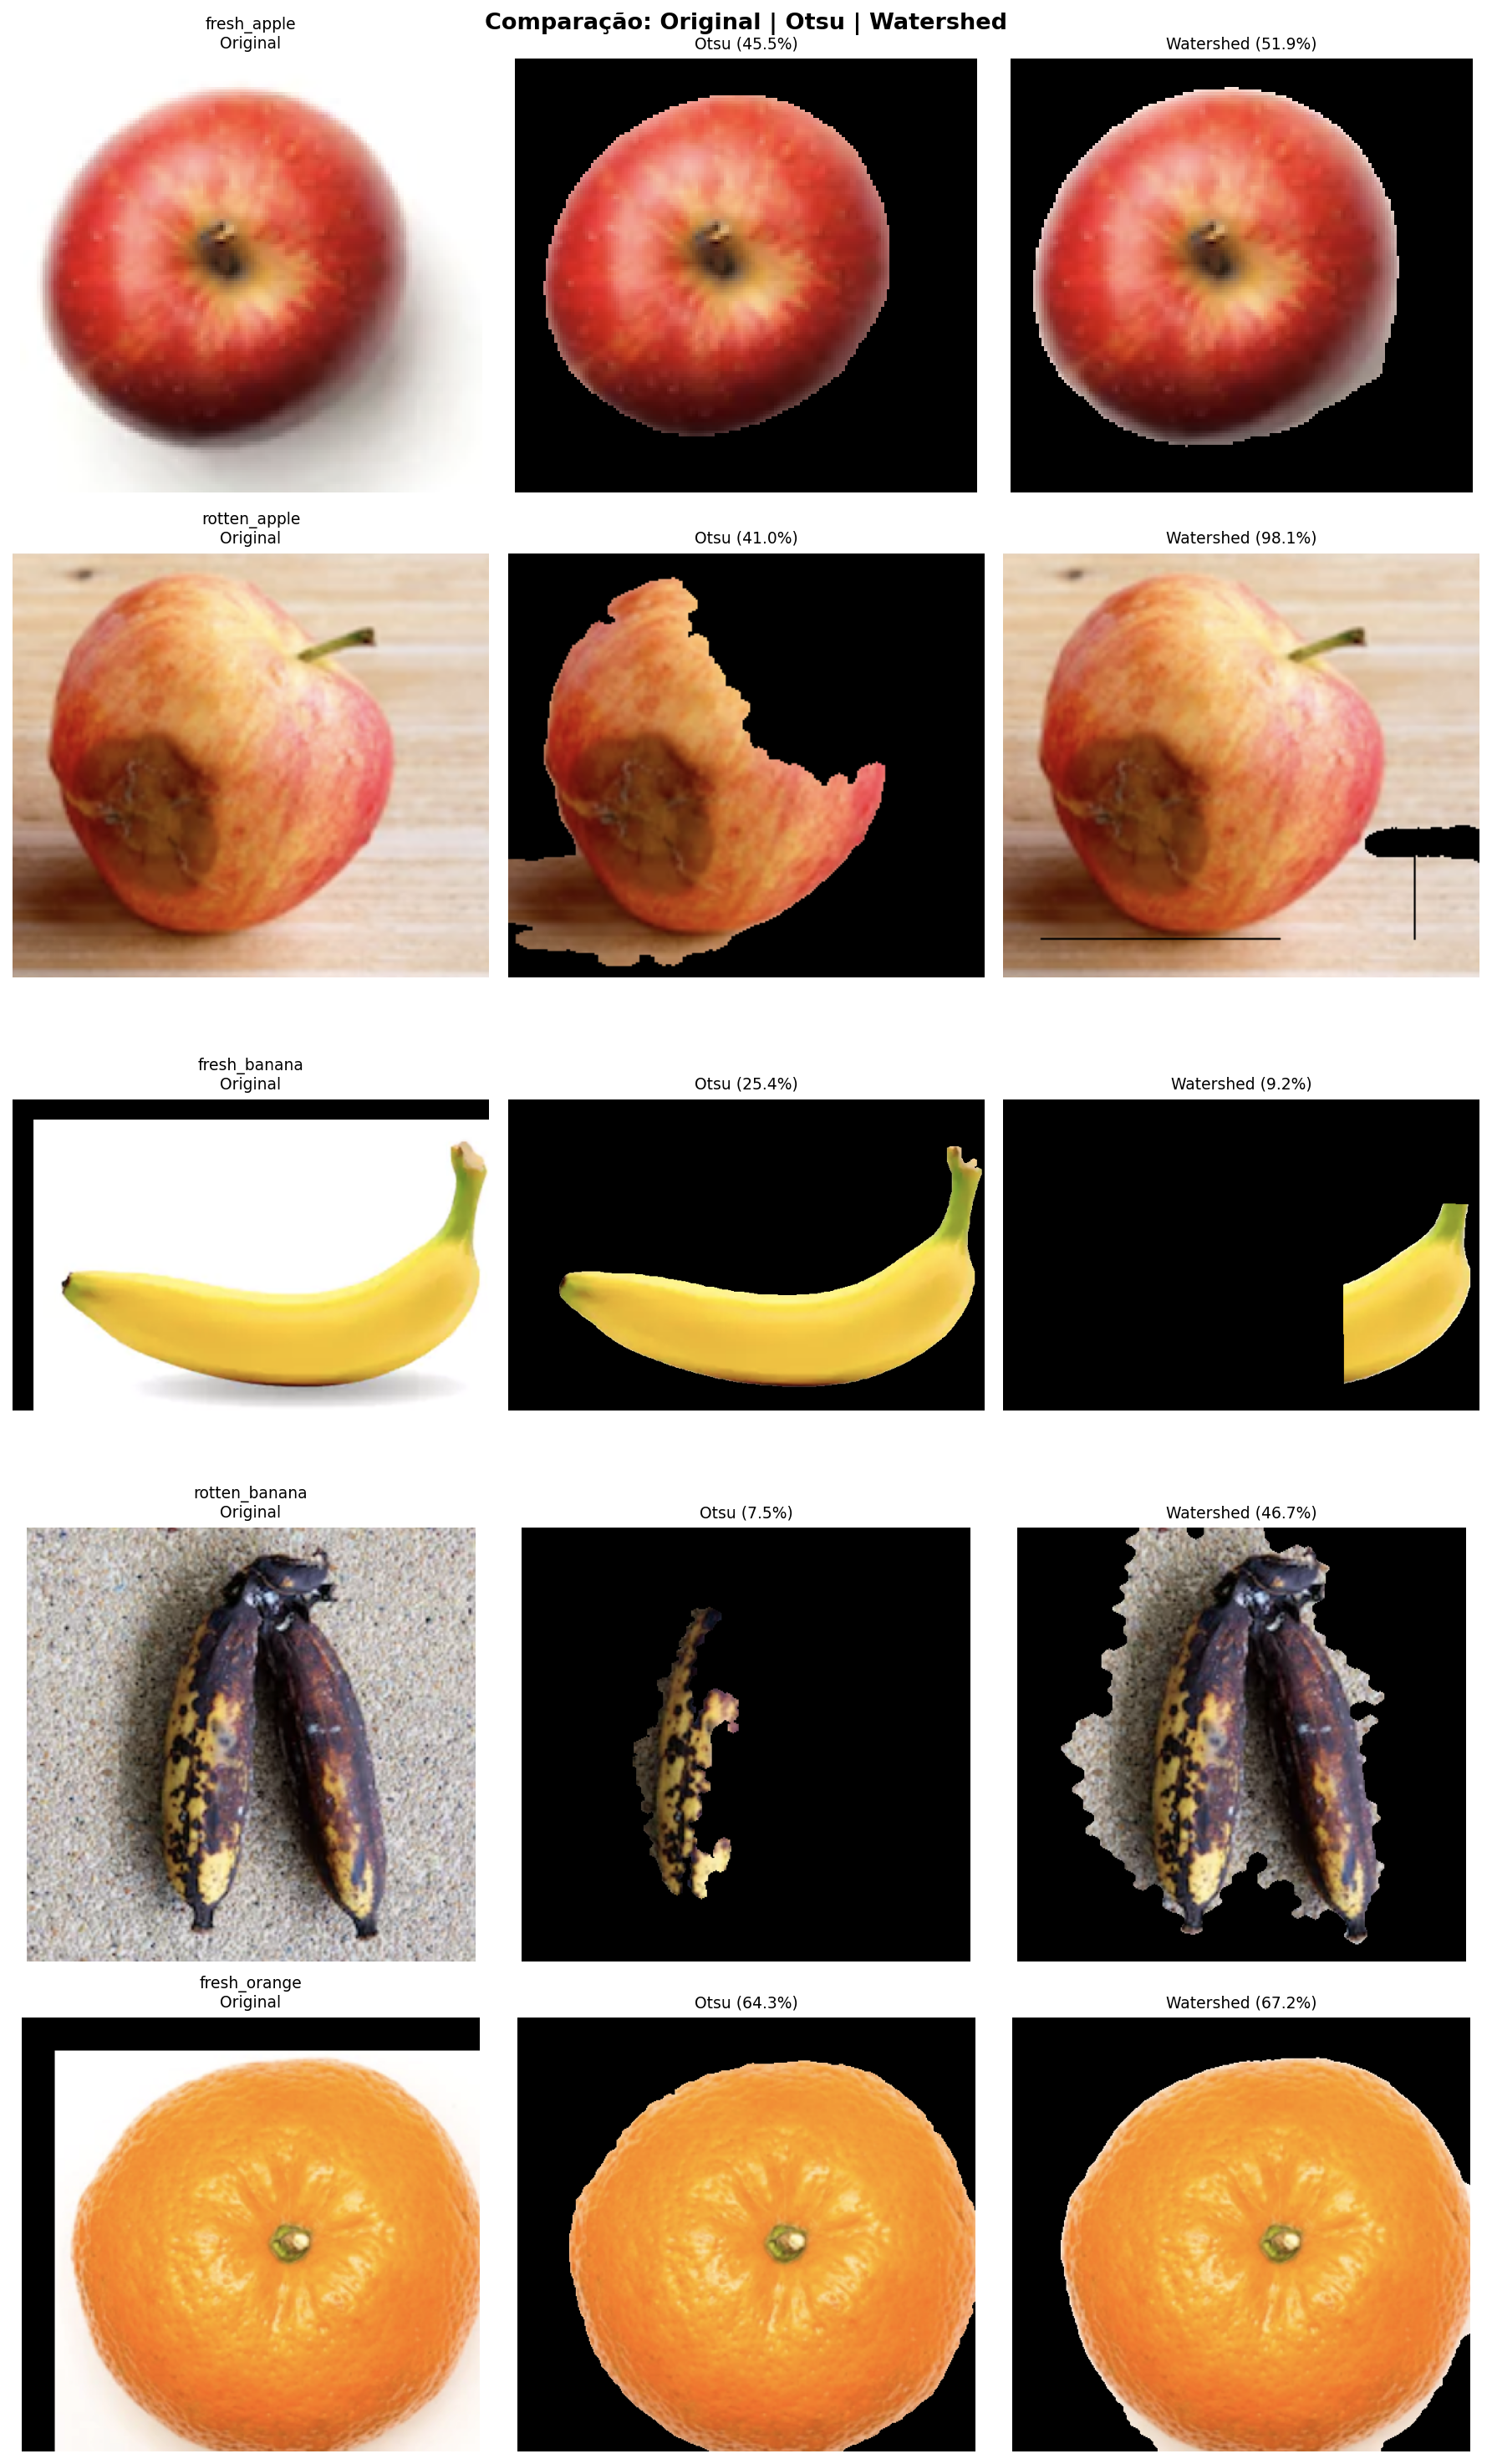
\includegraphics[width=0.92\textwidth]{../outputs/figures/seg_comparacao_metodos.png}
    \caption{Comparação: original, Otsu V2 e Watershed em imagens de classes mistas.}
    \label{fig:seg}
\end{figure}

% ============================================================
\section{Features Extraídas}
% ============================================================

Para cada imagem segmentada, extraímos \textbf{65 features} em 5 famílias.
A GLCM usou $\mathrm{distances}{=}[1]$ e ângulos $\{0°,45°,90°,135°\}$ (média das
4 direções para invariância direcional). O LBP usou $P{=}24$, $R{=}3$,
método \texttt{uniform} (26 bins).

\begin{table}[!htbp]
\centering
\caption{Famílias de features extraídas por imagem segmentada.}
\label{tab:features}
\small
\begin{tabular}{p{2.4cm} c p{4.6cm} p{4.6cm}}
\toprule
\textbf{Família} & \textbf{N} & \textbf{Features} & \textbf{Justificativa} \\
\midrule
Forma & 6 &
    area, perimeter, eccentricity, solidity, extent, circularity &
    Podridão causa amassados e perda de volume. \\
Momentos Hu & 7 &
    $\mathrm{hu}_1\ldots\mathrm{hu}_7$ (escala log) &
    Invariantes a rotação, escala e translação. \\
Cor HSV & 22 &
    h/s/v mean e std; histograma matiz (16 bins) &
    Manchas e perda de saturação indicam deterioração. \\
Textura GLCM & 4 &
    contrast, homogeneity, energy, correlation &
    Mofo aumenta contraste e reduz energia. \\
Textura LBP & 26 &
    histograma normalizado (26 bins) &
    Padrões locais de casca complementam GLCM. \\
\midrule
\textbf{Total} & \textbf{65} & & \\
\bottomrule
\end{tabular}
\end{table}

% ============================================================
\section{Análise e Seleção de Features}
% ============================================================

\begin{figure}[!htbp]
    \centering
    \begin{subfigure}[b]{0.57\textwidth}
        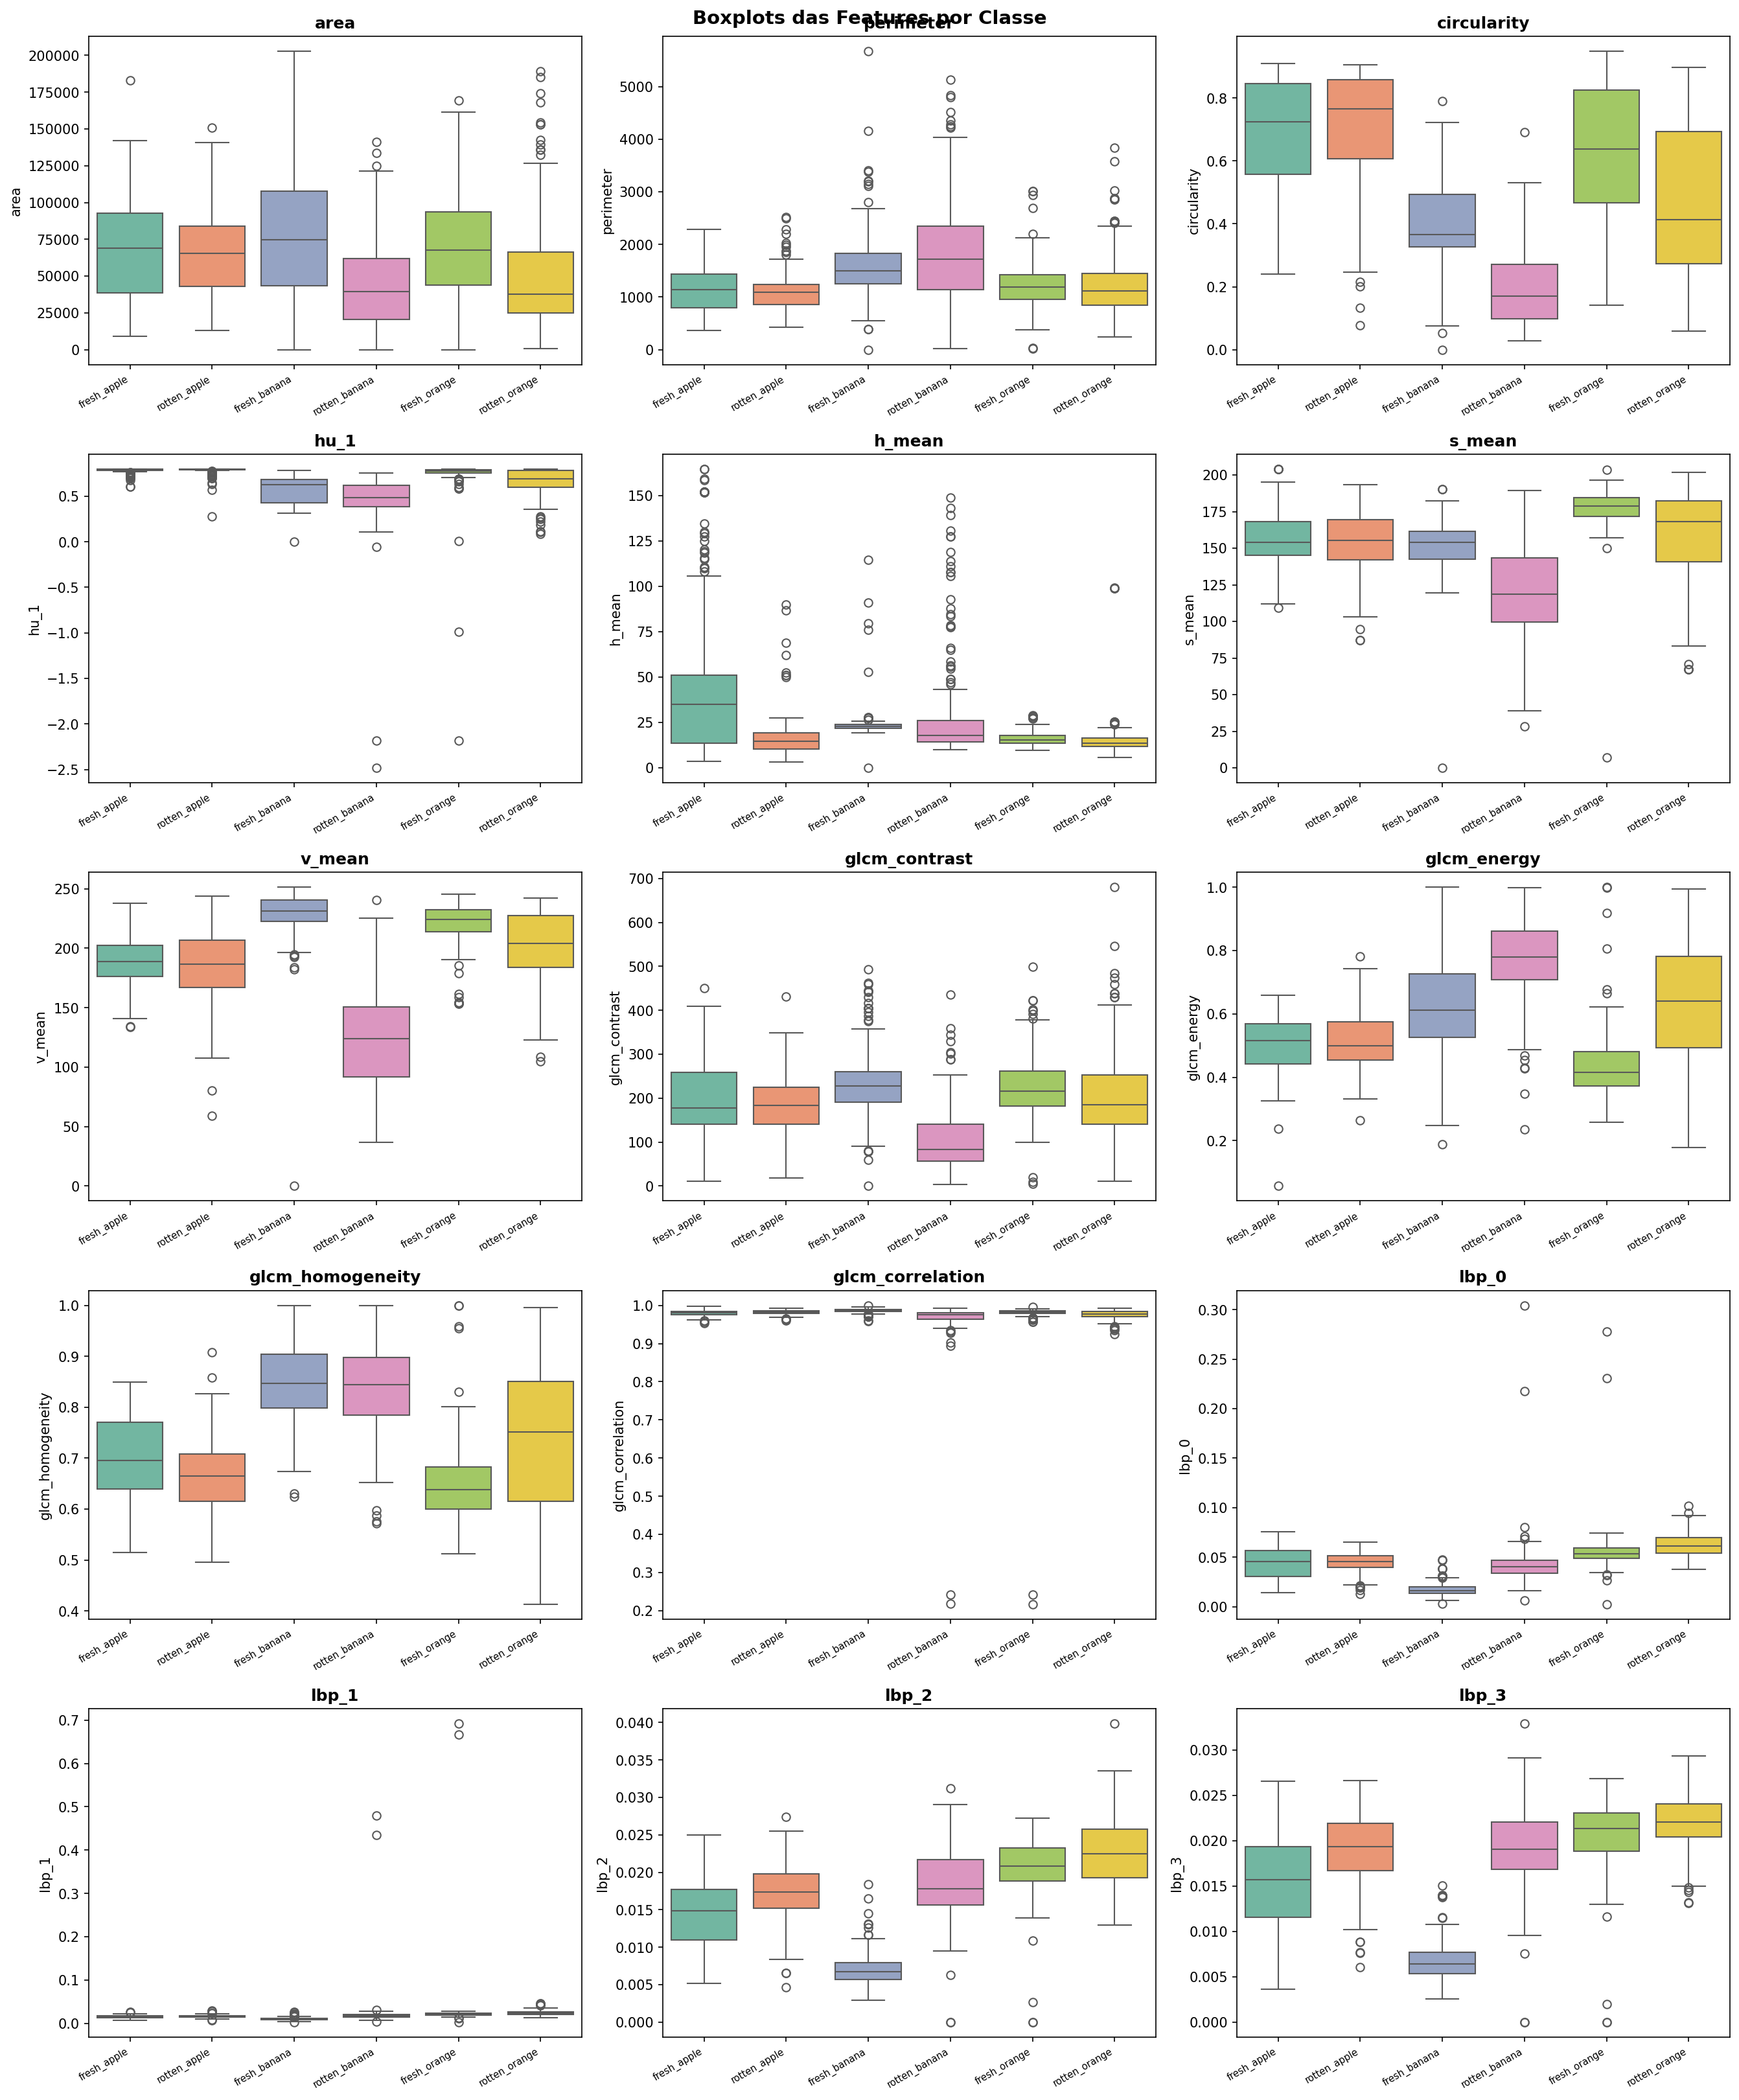
\includegraphics[width=\textwidth]{../outputs/figures/boxplots_por_classe.png}
        \caption{Boxplots das principais features por classe.}
        \label{fig:boxplots}
    \end{subfigure}
    \hfill
    \begin{subfigure}[b]{0.40\textwidth}
        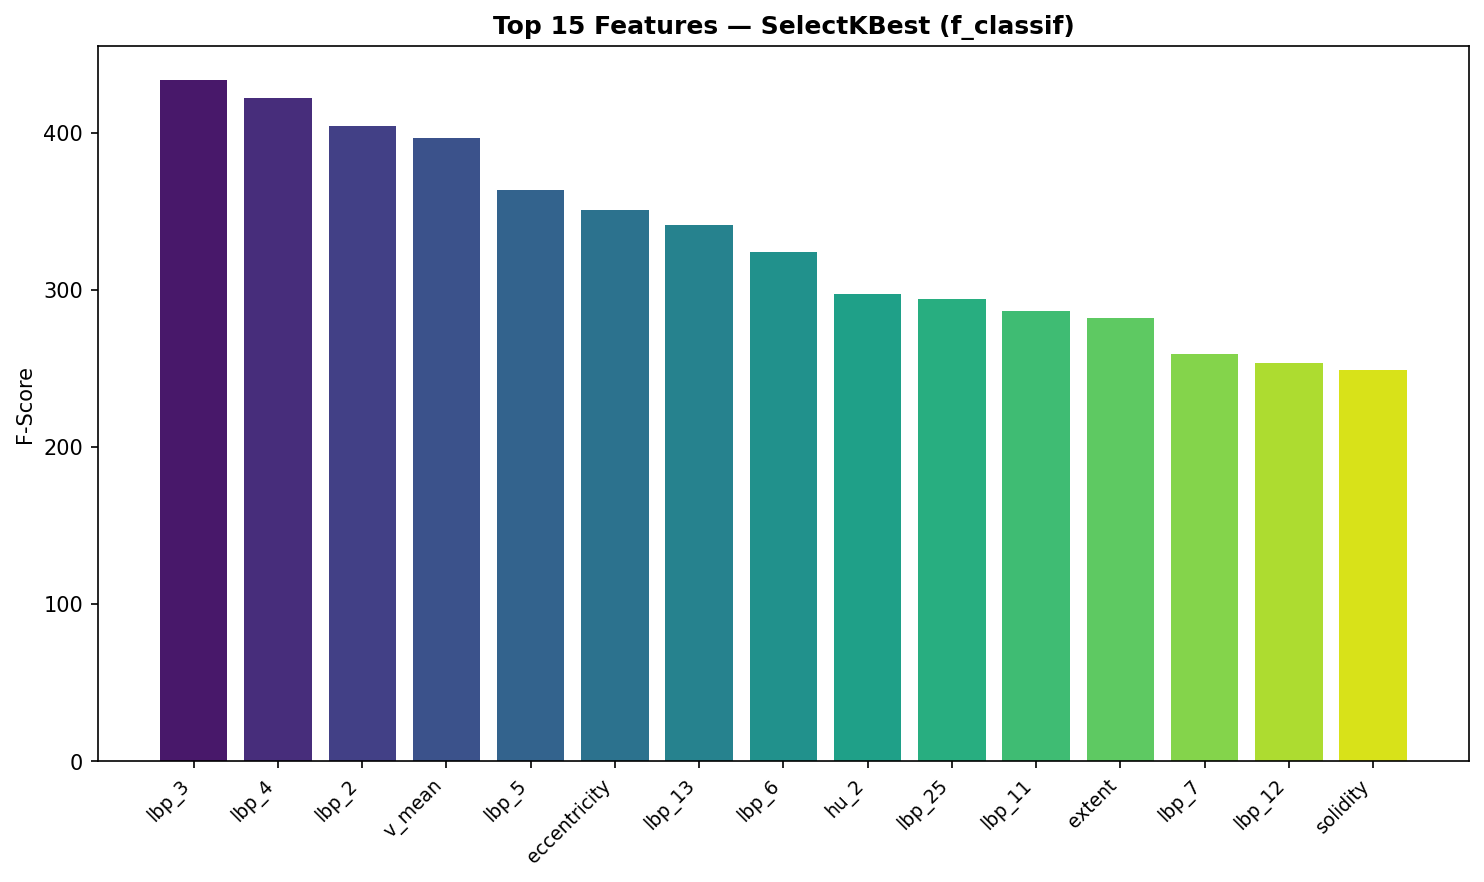
\includegraphics[width=\textwidth]{../outputs/figures/selectkbest_scores.png}
        \caption{Top features por F-score (SelectKBest).}
        \label{fig:skb}
    \end{subfigure}
    \caption{Distribuição por classe e ranking de relevância univariada das features.}
    \label{fig:feat_analysis}
\end{figure}

\texttt{v\_mean} e \texttt{h\_mean} separam claramente frutas frescas e podres.
SelectKBest elege como top~5: \texttt{lbp\_3}, \texttt{lbp\_4}, \texttt{lbp\_2},
\texttt{v\_mean}, \texttt{lbp\_5}. Importância RF: \texttt{v\_mean},
\texttt{h\_hist\_1}, \texttt{hu\_1}, \texttt{lbp\_3}, \texttt{h\_mean}.
Ambos destacam textura LBP e cor HSV.

\begin{figure}[!htbp]
    \centering
    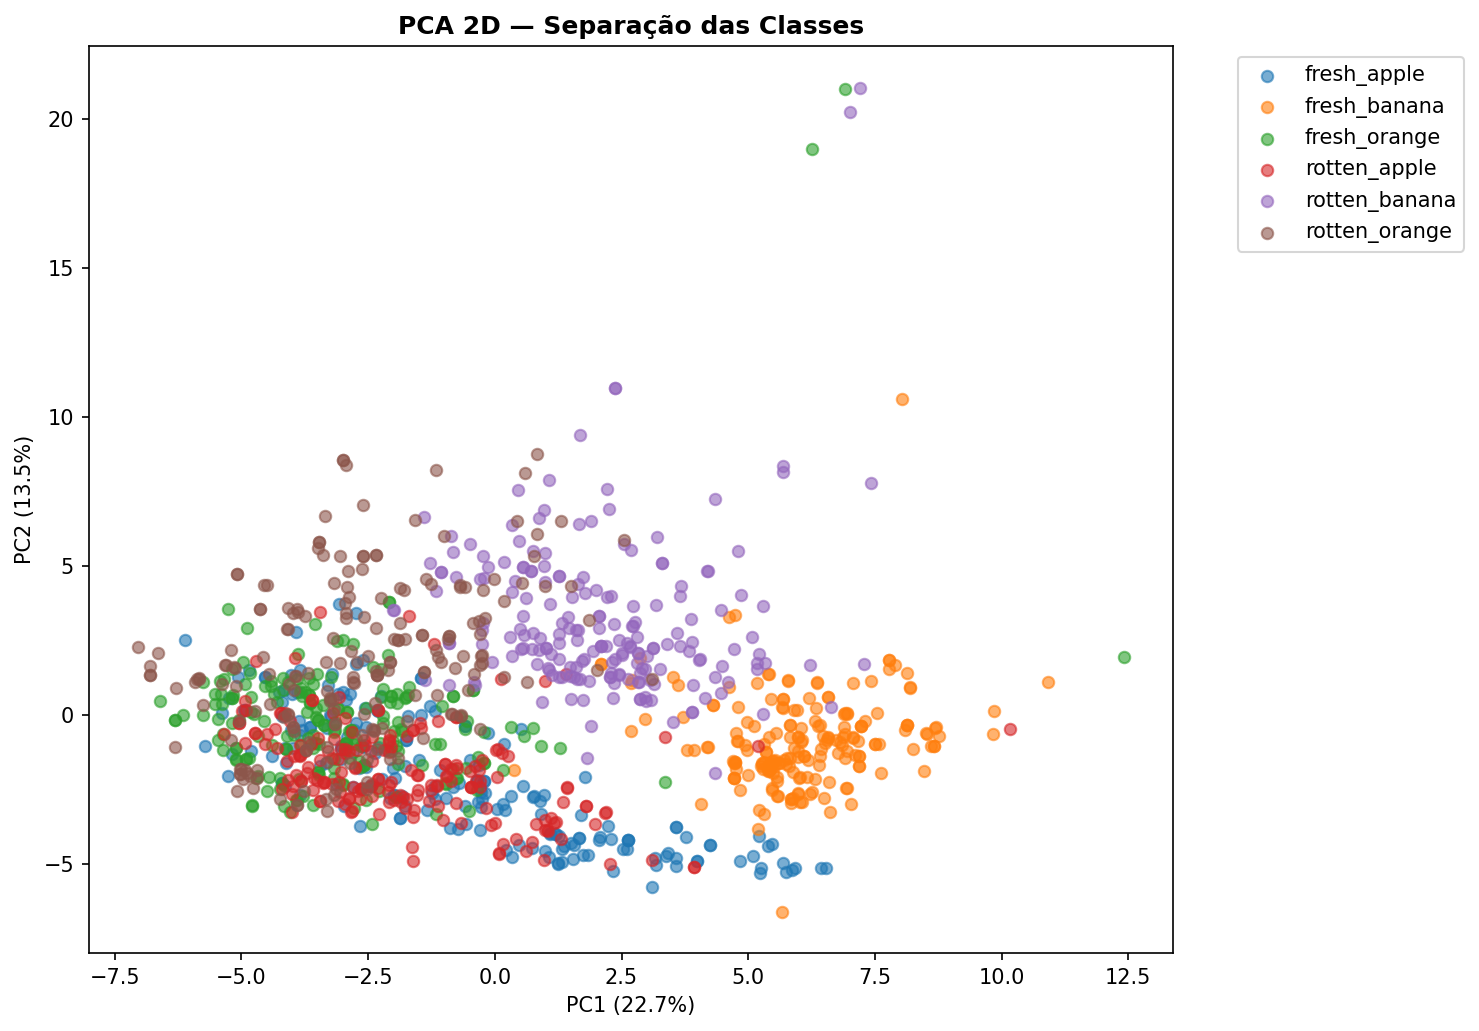
\includegraphics[width=0.60\textwidth]{../outputs/figures/pca_2d.png}
    \caption{PCA 2D (PC1=22,6\%, PC2=14,3\%; total 36,2\%). Agrupamentos parcialmente
             separados confirmam a discriminatividade das features.}
    \label{fig:pca}
\end{figure}

\textbf{Ablation Study:} treinamento com CV ($k{=}5$) em $X_{\mathrm{train}}$,
F1-macro por família:

\begin{figure}[!htbp]
    \centering
    \begin{subfigure}[b]{0.50\textwidth}
        \small
        \begin{tabular}{lrrr}
        \toprule
        \textbf{Grupo} & \textbf{LR} & \textbf{RF} & \textbf{SVM} \\
        \midrule
        G1: Cor (HSV)      & 0{,}643 & 0{,}831 & 0{,}742 \\
        G2: Textura        & 0{,}819 & 0{,}835 & 0{,}828 \\
        G3: Forma          & 0{,}532 & 0{,}660 & 0{,}556 \\
        \textbf{G4: Todos} & \textbf{0{,}906} & \textbf{0{,}912} & \textbf{0{,}900} \\
        \bottomrule
        \end{tabular}
        \vspace{0.3em}
        \caption{F1-macro por grupo (CV=5).}
    \end{subfigure}
    \hfill
    \begin{subfigure}[b]{0.46\textwidth}
        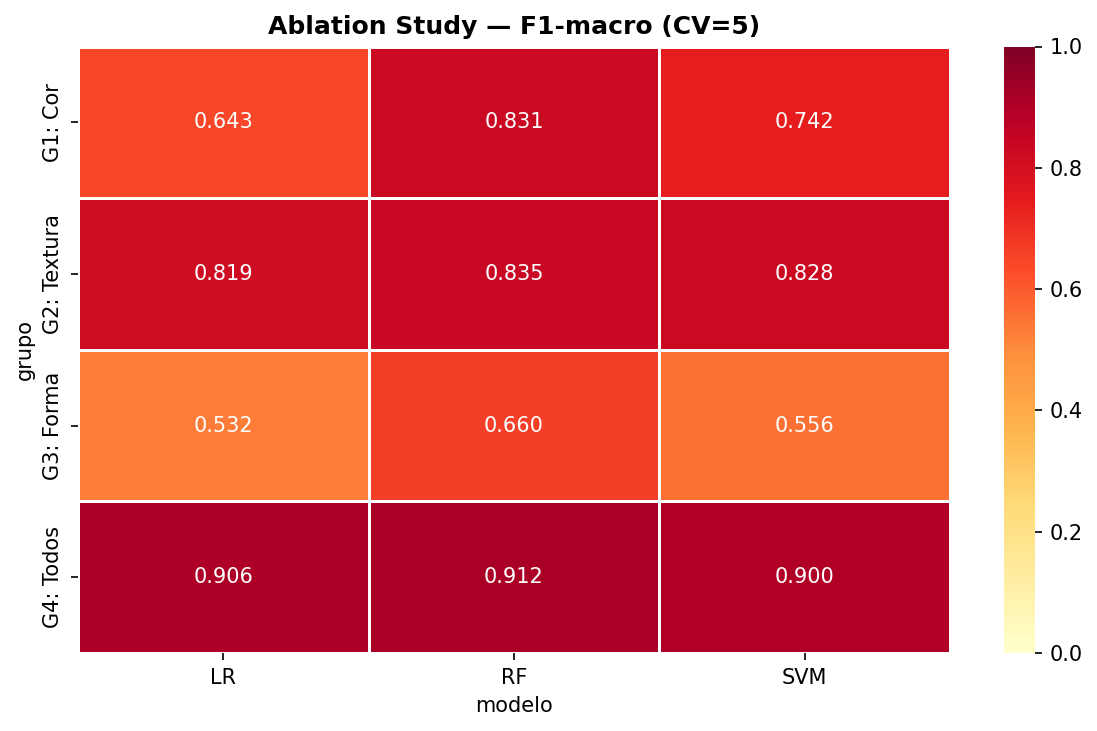
\includegraphics[width=\textwidth]{../outputs/figures/ablation_heatmap.png}
        \caption{Heatmap do ablation study.}
    \end{subfigure}
    \caption{Ablation study: contribuição de cada família de features.}
    \label{fig:ablation}
\end{figure}

Cor (G1) e textura (G2) são os grupos mais informativos isoladamente.
G4 supera o melhor grupo isolado em ${\approx}8\,\mathrm{pp}$ (RF: $0{,}831 \to 0{,}912$).
Forma (G3) tem menor poder discriminativo isolado.

\textbf{RFE:} Eliminação Recursiva com RF ($k{=}3$) selecionou \textbf{45 de 65 features}
sem perda mensurável. As 20 eliminadas são bins extremos do histograma de matiz e bins
LBP de baixa variância discriminativa.

% ============================================================
\section{Classificadores}
% ============================================================

Treinamos três classificadores clássicos: SVM com kernel RBF, Random Forest e
Regressão Logística. Para cada modelo, aplicamos \texttt{GridSearchCV} com
\texttt{StratifiedKFold} ($k{=}5$) sobre o conjunto treino+validação, usando
F1-macro como métrica de seleção. O conjunto de teste foi mantido isolado em
toda essa etapa. A Tabela~\ref{tab:classif} apresenta os espaços de busca e
os melhores hiperparâmetros encontrados.

\begin{table}[!htbp]
\centering
\caption{Configuração e melhores hiperparâmetros dos classificadores (\texttt{GridSearchCV},
         \texttt{StratifiedKFold} $k{=}5$, métrica \texttt{f1\_macro}).}
\label{tab:classif}
\small
\begin{tabular}{p{2.2cm} p{2.8cm} p{5.0cm} p{2.8cm}}
\toprule
\textbf{Modelo} & \textbf{Biblioteca} & \textbf{Espaço de busca} & \textbf{Melhor config.} \\
\midrule
SVM &
\texttt{SVC} &
C $\in\{0.1,1,10,100\}$; kernel $\in\{\mathrm{rbf,linear}\}$; gamma $\in\{\mathrm{scale,auto}\}$ &
C=10, rbf, scale \\
Random Forest &
\texttt{RandomForest\-Classifier} &
n\_est $\in\{100,200\}$; max\_depth $\in\{\mathrm{None},10,20\}$; min\_split $\in\{2,5\}$ &
n\_est=200, depth=None, split=2 \\
Log.\ Regression &
\texttt{Logistic\-Regression} &
C $\in\{0.01,0.1,1,10\}$; penalty $\in\{\ell_1,\ell_2\}$; solver=liblinear &
C=10, $\ell_1$, liblinear \\
\bottomrule
\end{tabular}
\end{table}

% ============================================================
\section{Resultados e Métricas}
% ============================================================

\begin{table}[!htbp]
\centering
\caption{Resultados no test set (15\% estratificado, 180 amostras).}
\label{tab:results}
\small
\begin{tabular}{lrrrrr}
\toprule
\textbf{Modelo} & \textbf{Acc.} & \textbf{Prec.} & \textbf{Rec.} & \textbf{F1-macro} & \textbf{AUC} \\
\midrule
\textbf{Random Forest} \textit{(melhor clássico)} &
    \textbf{95{,}00\%} & \textbf{95{,}00\%} & \textbf{95{,}00\%} & \textbf{0{,}950} & \textbf{0{,}9951} \\
SVM (RBF, C=10) &
    93{,}89\% & 94{,}18\% & 93{,}89\% & 0{,}939 & 0{,}9930 \\
Log.\ Regression ($\ell_1$, C=10) &
    91{,}11\% & 91{,}12\% & 91{,}11\% & 0{,}910 & 0{,}9900 \\
\textbf{MobileNetV2} \textit{(bônus)} &
    \textbf{97{,}22\%} & \textbf{97{,}40\%} & \textbf{97{,}22\%} & \textbf{0{,}972} & {*} \\
\bottomrule
\end{tabular}
\end{table}
{\small * AUC não calculado para MobileNetV2 (one-vs-rest aplicado apenas aos modelos clássicos).}

Validação cruzada ($k{=}5$) em $X_{\mathrm{train}}$:
SVM $0{,}945\pm0{,}014$, RF $0{,}928\pm0{,}010$, LR $0{,}923\pm0{,}012$.
Baixas variâncias confirmam estabilidade.

\begin{figure}[!htbp]
    \centering
    \begin{subfigure}[b]{0.48\textwidth}
        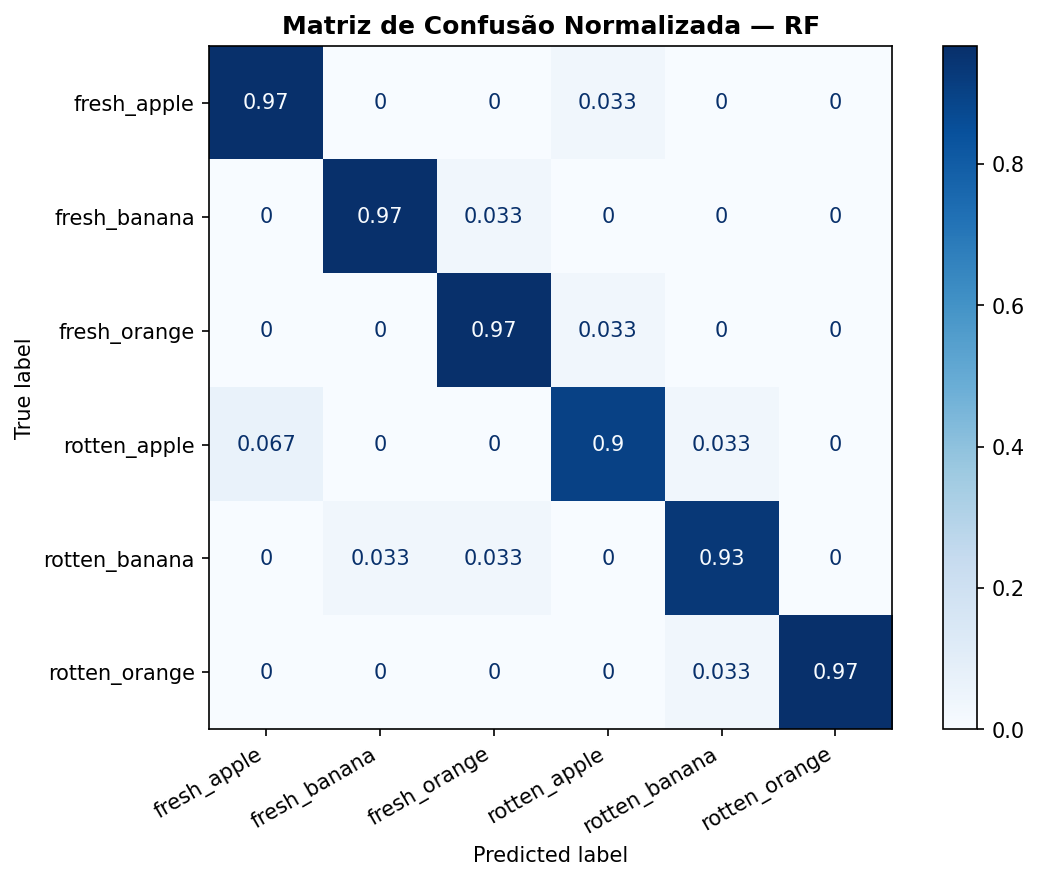
\includegraphics[width=\textwidth]{../outputs/figures/cm_rf.png}
        \caption{Matriz de confusão do RF (9/180 erros).}
    \end{subfigure}
    \hfill
    \begin{subfigure}[b]{0.48\textwidth}
        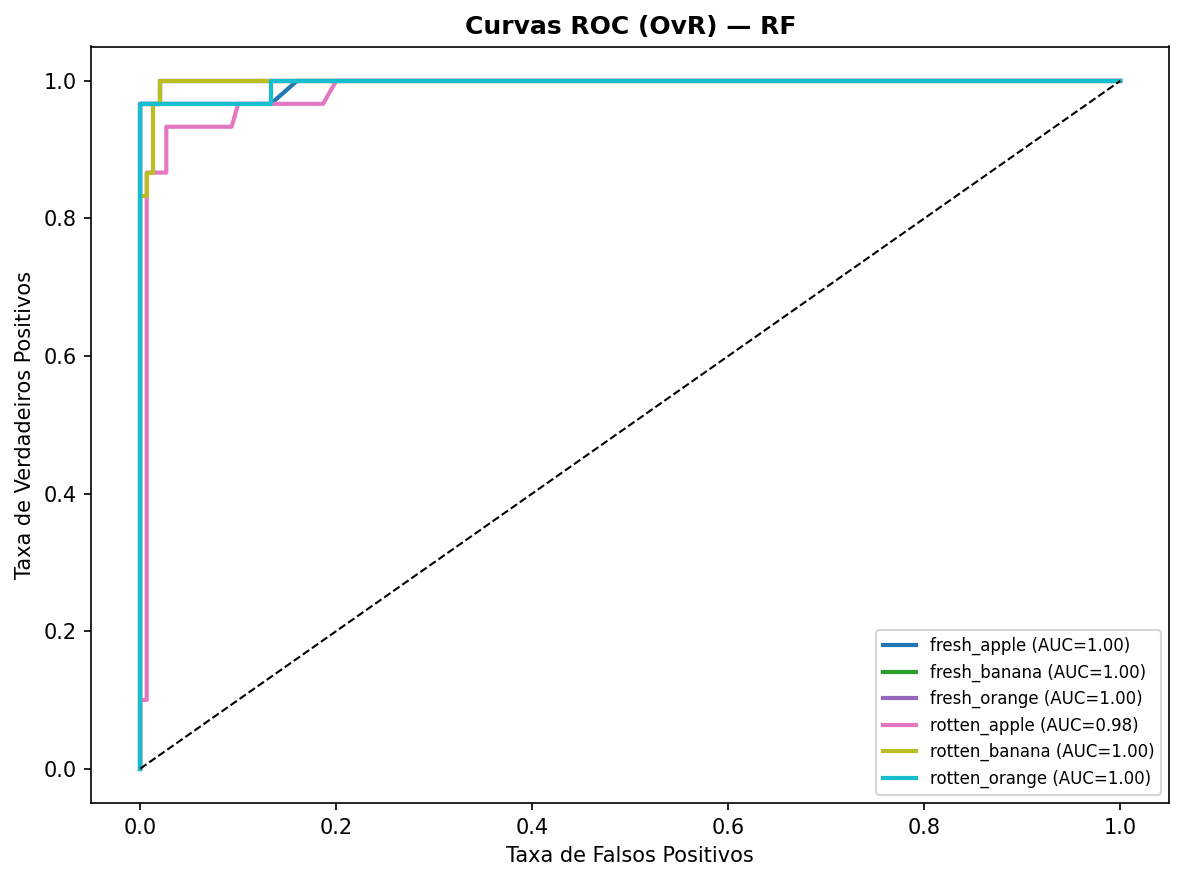
\includegraphics[width=\textwidth]{../outputs/figures/roc_rf.png}
        \caption{Curvas ROC one-vs-rest do RF.}
    \end{subfigure}
    \caption{Avaliação do Random Forest (melhor clássico) no test set.}
    \label{fig:rf_eval}
\end{figure}

\begin{figure}[!htbp]
    \centering
    \begin{subfigure}[b]{0.48\textwidth}
        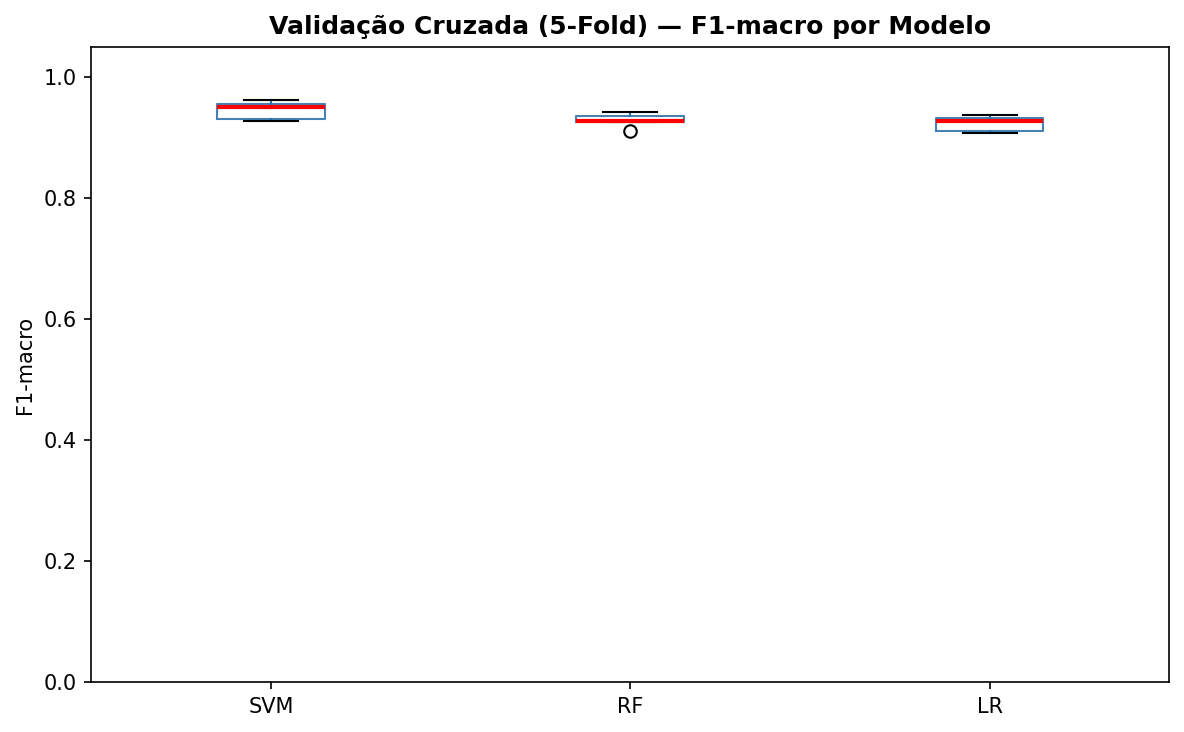
\includegraphics[width=\textwidth]{../outputs/figures/crossval_boxplot.png}
        \caption{F1-macro por fold (CV=5, $X_{\mathrm{train}}$).}
    \end{subfigure}
    \hfill
    \begin{subfigure}[b]{0.48\textwidth}
        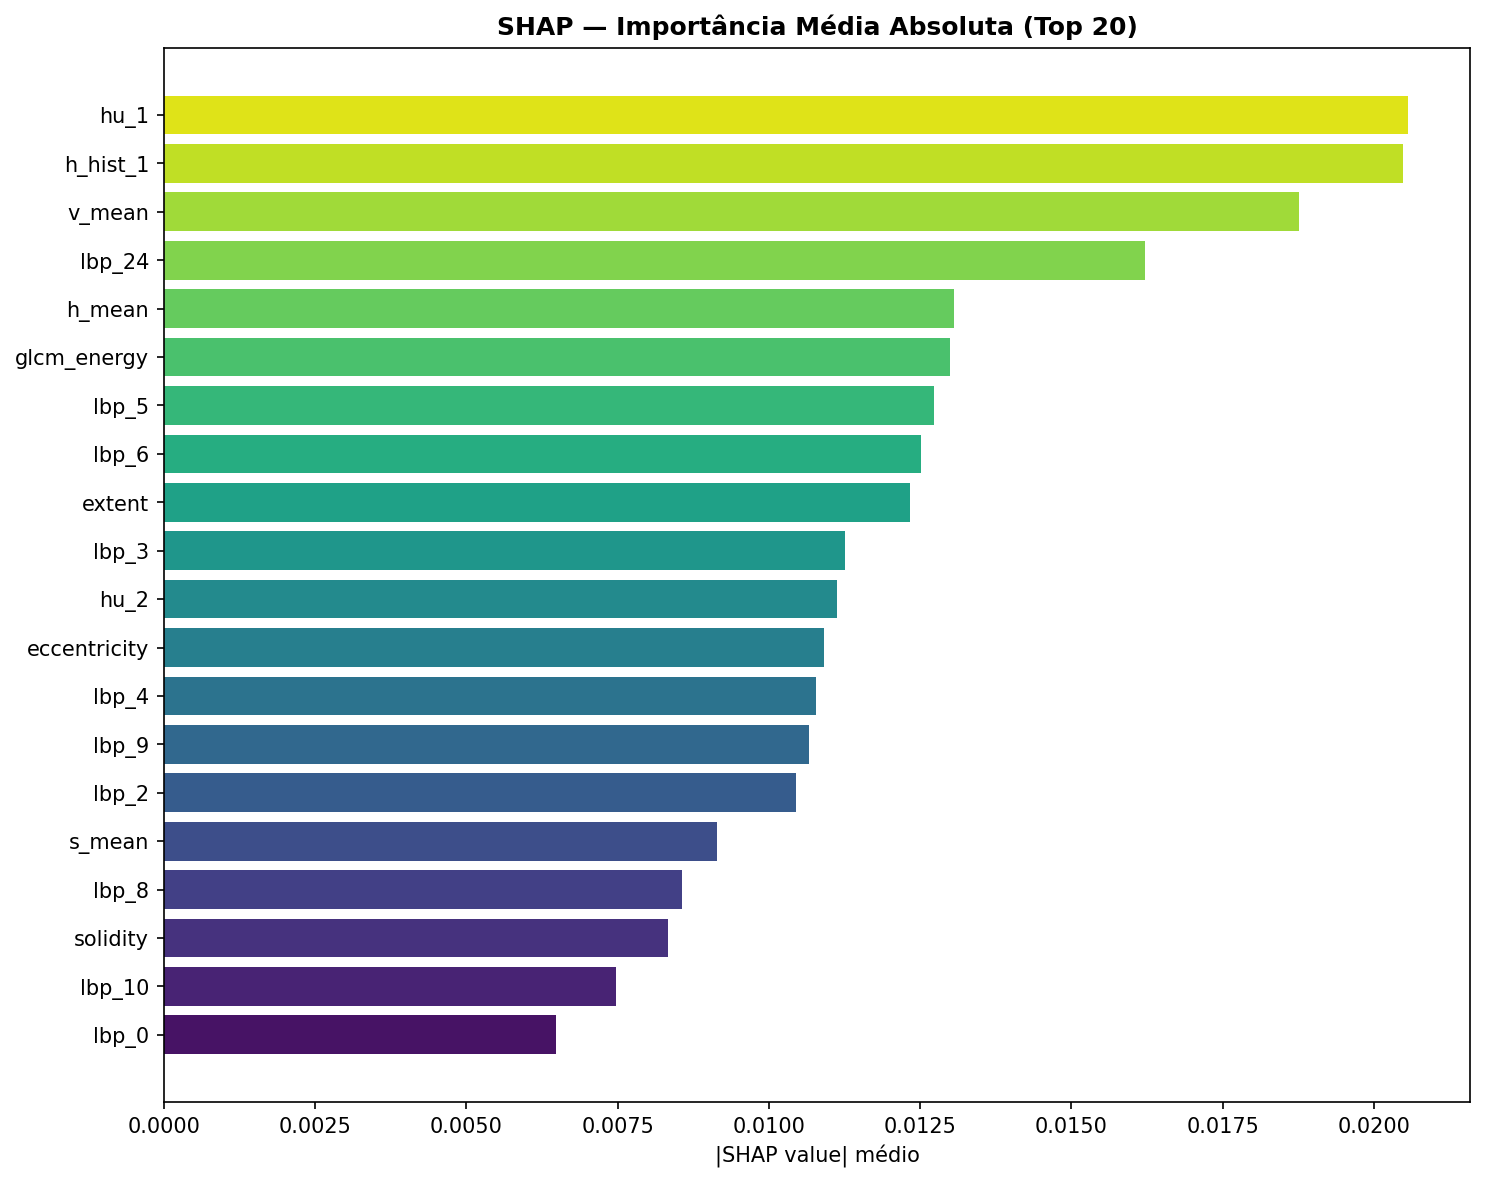
\includegraphics[width=\textwidth]{../outputs/figures/shap_bar.png}
        \caption{Importância SHAP absoluta média do RF (top 20).}
    \end{subfigure}
    \caption{Estabilidade (validação cruzada) e interpretabilidade (SHAP).
             \texttt{v\_mean} e \texttt{h\_mean} dominam as predições, resultado coerente com o domínio.}
    \label{fig:cv_shap}
\end{figure}

% ============================================================
\section{Análise de Erros}
% ============================================================

\begin{figure}[!htbp]
    \centering
    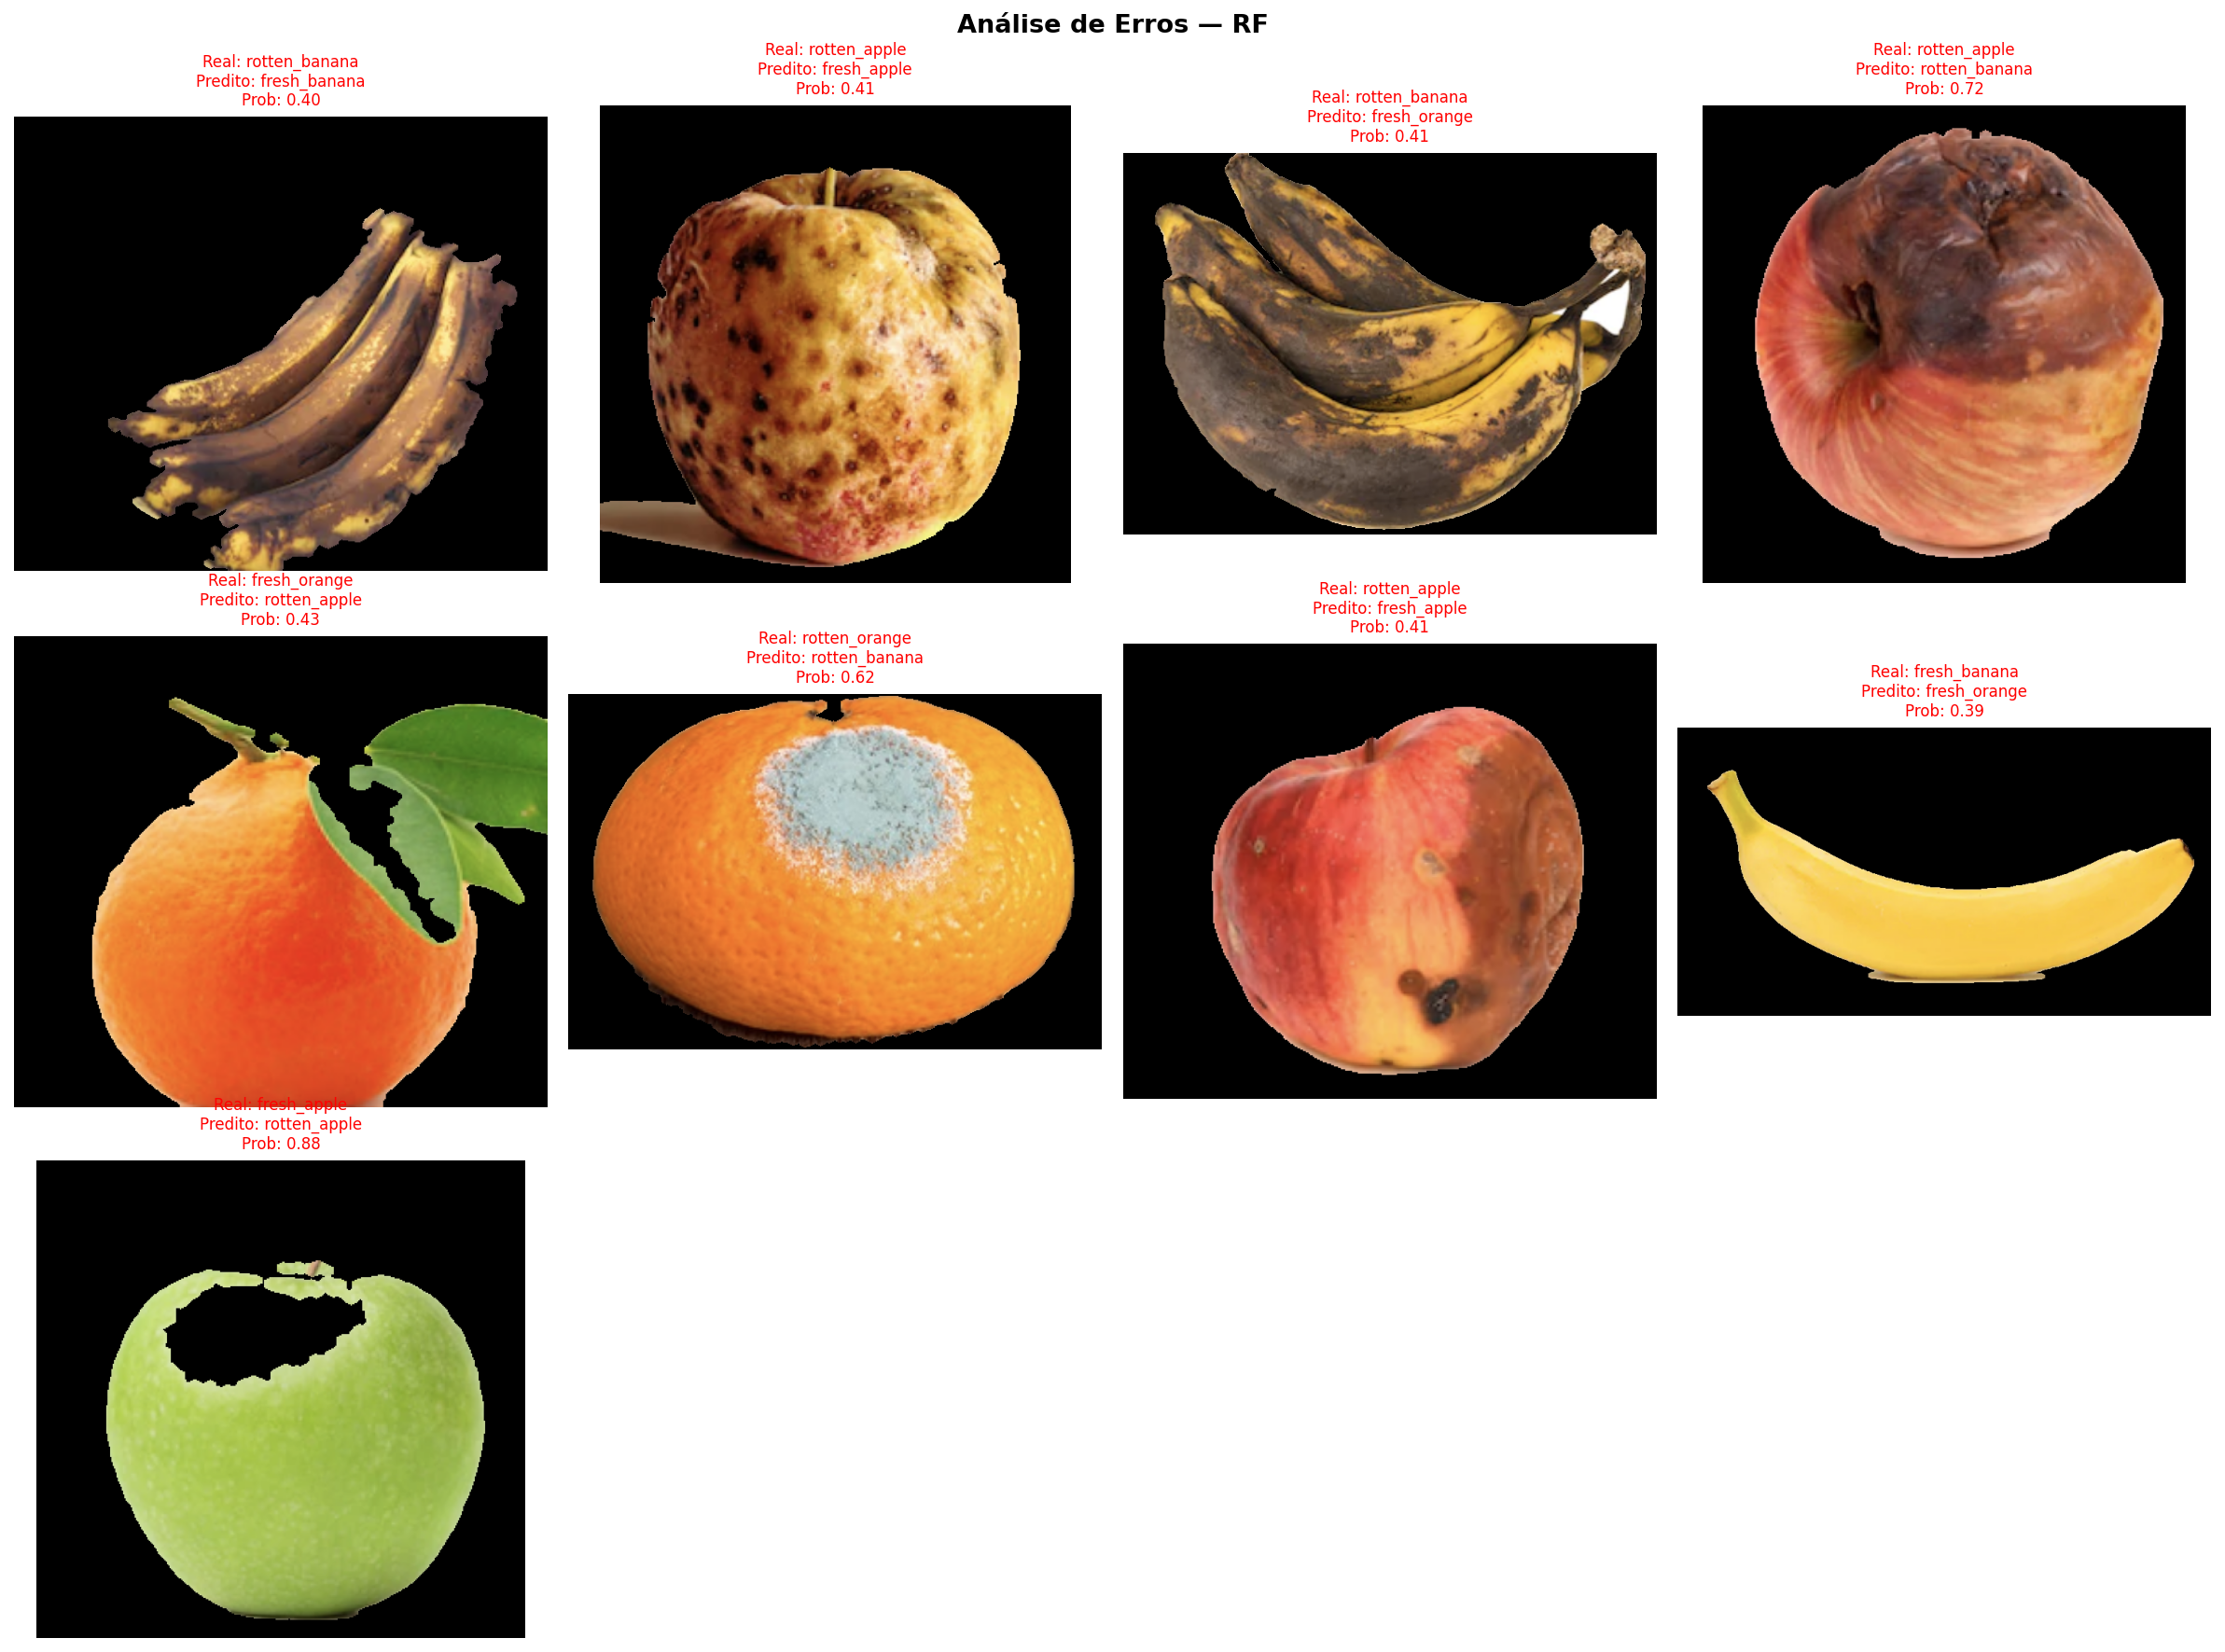
\includegraphics[width=0.88\textwidth]{../outputs/figures/analise_erros.png}
    \caption{Exemplos de erros do Random Forest no test set (classe real vs.\ predita).}
    \label{fig:erros}
\end{figure}

O RF comete 9 erros; a classe mais difícil é \texttt{rotten\_apple}
(recall\,$=\,0{,}90$; 3 erros). Hipóteses:
(1)~maçãs com oxidação inicial apresentam coloração intermediária, enganando features de cor;
(2)~sombras difusas elevam \texttt{glcm\_contrast} e reduzem \texttt{s\_mean}, induzindo
falsos positivos;
(3)~reflexo especular altera \texttt{h\_mean} e \texttt{v\_mean} (as features de maior
peso SHAP);
(4)~bananas maduras com manchas naturais se assemelham a \texttt{rotten\_banana} pelo
histograma de matiz.

% ============================================================
\section{Conclusão}
% ============================================================

\begin{itemize}\setlength{\itemsep}{0pt}
    \item O \textbf{Random Forest} atingiu F1-macro $= 0{,}950$ (AUC $= 0{,}9951$),
          melhor resultado clássico; adequado para CPU embarcada com interpretabilidade via SHAP.
    \item Entre as famílias de features, \textbf{cor HSV} se destaca individualmente
          (RF: F1 $= 0{,}831$); textura LBP aparece como segunda mais discriminativa
          segundo SHAP e SelectKBest.
    \item A \textbf{combinação completa} (G4) supera o melhor grupo isolado em
          ${\approx}8\,\mathrm{pp}$, confirmando sinergia entre cor, textura e forma.
    \item \textbf{MobileNetV2} supera os clássicos em $+2{,}2\,\mathrm{pp}$ de F1-macro
          ($0{,}972$ vs.\ $0{,}950$), ao custo de maior complexidade computacional e
          menor interpretabilidade direta.
    \item Para \textbf{máxima acurácia com GPU}: MobileNetV2 com Grad-CAM.
          Para \textbf{CPU embarcada}: RF com o pipeline clássico.
\end{itemize}

% ============================================================
\section{Bônus e Discussão Avançada}
% ============================================================

{\small
\textbf{MobileNetV2 (Transfer Learning):}
Treinamento em duas fases: (1)~backbone ImageNet congelado; cabeça
(\texttt{GAP}$\!\to\!$\texttt{Dropout}(0,3)$\!\to\!$\texttt{Dense}(128)$\!\to\!$\texttt{Softmax}(6))
por 10 épocas (\texttt{Adam}, lr$=10^{-3}$);
(2)~fine-tuning dos últimos 30 layers por 10 épocas (\texttt{Adam}, lr$=10^{-4}$).
Acurácia de treino $= 1{,}000$ e validação $\approx 0{,}975$ indicam
\textbf{overfitting leve} (${\approx}2{,}5\,\mathrm{pp}$), esperado com apenas
${\approx}840$ imagens de treino.
}

\begin{figure}[!htbp]
    \centering
    \begin{subfigure}[b]{0.47\textwidth}
        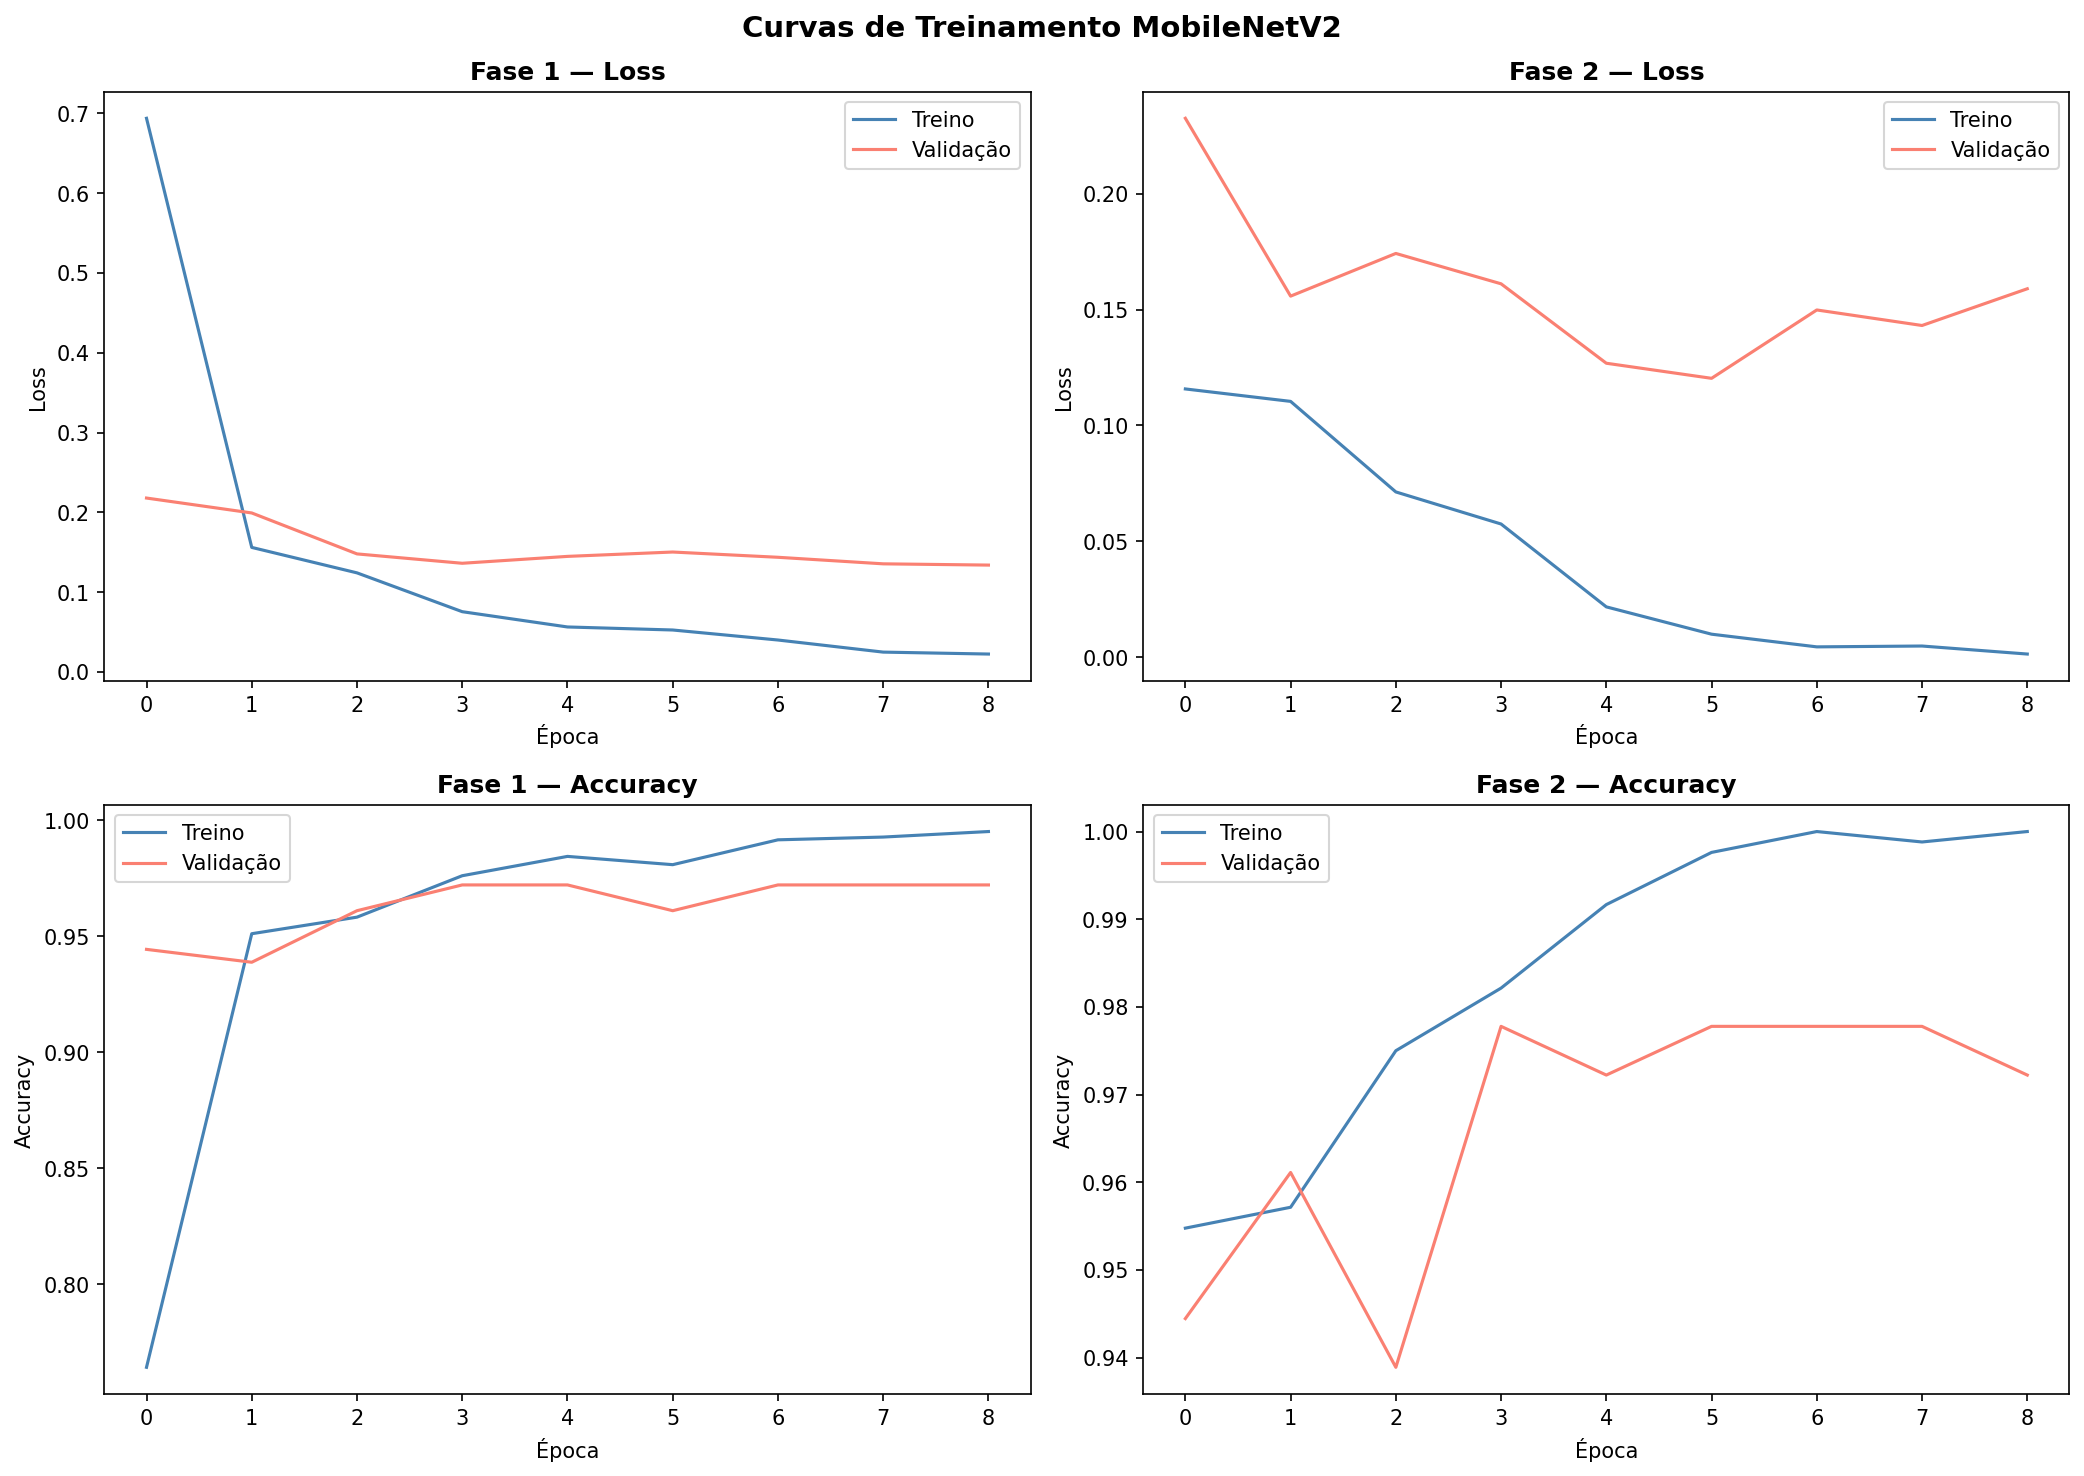
\includegraphics[width=\textwidth,height=4.2cm,keepaspectratio]{../outputs/figures/cnn_training_curves.png}
        \caption{Curvas de treino e validação (fases 1 e 2).}
    \end{subfigure}
    \hfill
    \begin{subfigure}[b]{0.47\textwidth}
        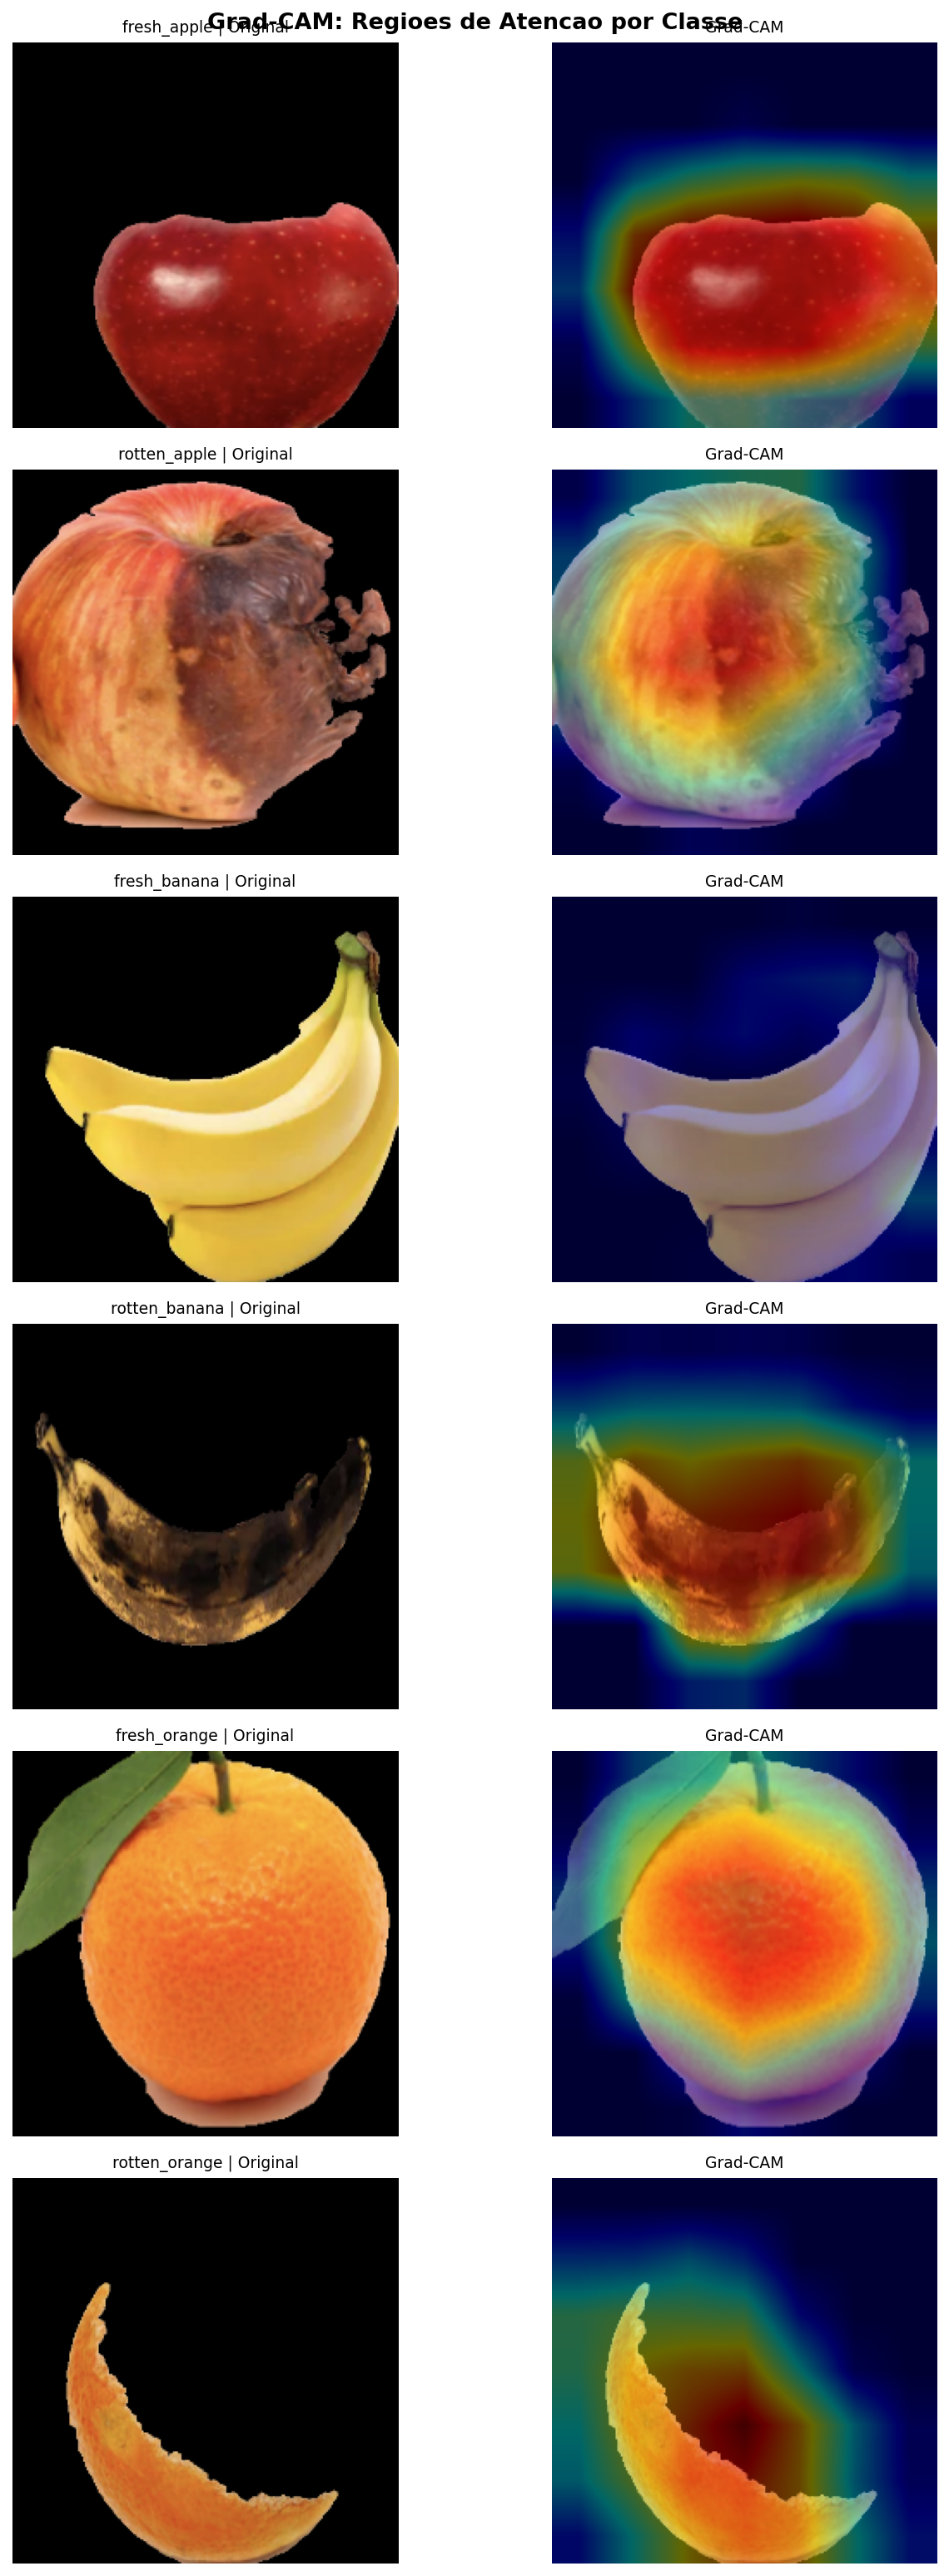
\includegraphics[width=\textwidth,height=4.2cm,keepaspectratio]{../outputs/figures/gradcam_exemplos.png}
        \caption{Grad-CAM: regiões de atenção por classe.}
    \end{subfigure}
    \caption{MobileNetV2: dinâmica de treinamento e interpretabilidade Grad-CAM.}
    \label{fig:cnn}
\end{figure}

{\small
\textbf{Discussão do Data Leakage:}
O dataset Kaggle continha variantes augmentadas (rotações de 15°, 30° e ruído
\textit{salt-and-pepper}). Um split aleatório sem agrupamento vazava ${\approx}62\%$
das amostras de teste para o treino. Removemos as variantes e revalidamos via pHash
(${\leq}0{,}5\%$ de pares residuais). As features clássicas (Hu, HSV média, GLCM
com média de 4 ângulos) são majoritariamente \textbf{invariantes à rotação}: o
leakage por rotação contribuía redundância, não informação nova, afetando pouco o
pipeline clássico. A CNN, que opera sobre pixels, era mais suscetível; contudo, a
queda foi de apenas $0{,}5\,\mathrm{pp}$ em F1-macro, atribuível à robustez do
backbone ImageNet e ao tamanho limitado do test set (180 amostras).

\textbf{Demais contribuições:}
\textit{SHAP (TreeExplainer):} interpretação quantitativa das predições do RF, alinhada ao domínio.
\textit{Ablation study:} 4 grupos $\times$ 3 modelos com CV=5, quantificando contribuição marginal de cada família.
\textit{RFE:} redução de 65 para 45 features sem perda mensurável.
\textit{Streamlit:} interface web com upload de imagem, segmentação e predição em tempo real.
}

\end{document}
